%% This is an example first chapter.  You should put chapter/appendix that you
%% write into a separate file, and add a line \include{yourfilename} to
%% main.tex, where `yourfilename.tex' is the name of the chapter/appendix file.
%% You can process specific files by typing their names in at the 
%% \files=
%% prompt when you run the file main.tex through LaTeX.
\chapter{Results}

\section{Perturation of States}
\label{sec:perturbation_of_states}
Early attempts at running the DSHKEnKF on the hydrologic model were marked by the complete collapse of posterior ensemble covariance to the mean and erratic jumps from the minimum to the maximum bounds for all streamflow parameters. Snow water equivalent parameters and states, however, converged in a stable fashion. It was determined that these erratic jumps were due to the hydrologic model's dependence on the value of the catchments' lowest groundwater reservoir, an unobserved and uncorrected state, which was integral to the production of streamflow in each timestep. White noise added to the forcing data (precipitation and min/max temperature) was unable to generate adequately diverse ensemble behavior when groundwater states were uniform across ensembles. To account for this, perturbation of groundwater and streamflow states was implemented.

\subsection{Perturbation of Groundwater States}

The hydrologic model was extremely sensitive to its starting states, in particular the lower groundwater reservoir. A low groundwater would lead to underwhelming groundwater, incentivising the parameters \texttt{ck0}, \texttt{ck1}, and \texttt{ck2} to converge towards values that emptied all water pouring into the reservoirs so modeled streamflow could match the observations. Conversely, high starting groundwater caused \texttt{ck0}, \texttt{ck1}, and \texttt{ck2} to converge towards parameters that let very little groundwater out of the reservoirs, further exasperating the problem and causing higher and higher values for \texttt{ck0}, \texttt{ck1}, and \texttt{ck2} to be chosen. 

To solve this issue and find a reliable blanket starting value for groundwater subcatchments in an efficient amount of time the small dataset was utilized alongside the parameter boundaries specified by \cite{Maneta2008}. Trial and error was utilized on the dataset until groundwater stabilized. To encourage the model to explore different parameter values for different amounts of groundwater, initial states for the large dataset were perturbed across all ensembles and catchments using a $\mu$ equal to the average stable value of the small dataset, which for this model was roughly calculated to be 100mm, and a $\sigma$ of 80mm. During the prediction phase groundwater was treated as forcing data and was perturbed slightly at a $\sigma$ of $u_{gw} * gw$, with $u_{gw}$  at .05%.

\begin{figure}
\centering
\begin{minipage}{.5\textwidth}
  \centering
  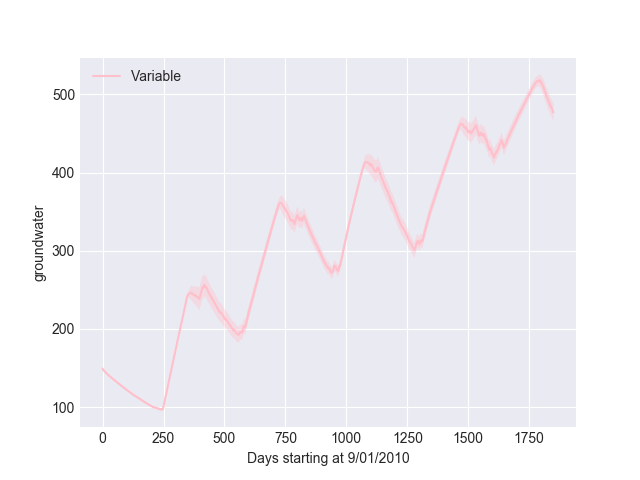
\includegraphics[width=.98\linewidth]{bad_gw}
  \captionof{figure}{Uniform groundwater}
  \label{fig:bad_gw}
\end{minipage}%
\begin{minipage}{.5\textwidth}
  \centering
  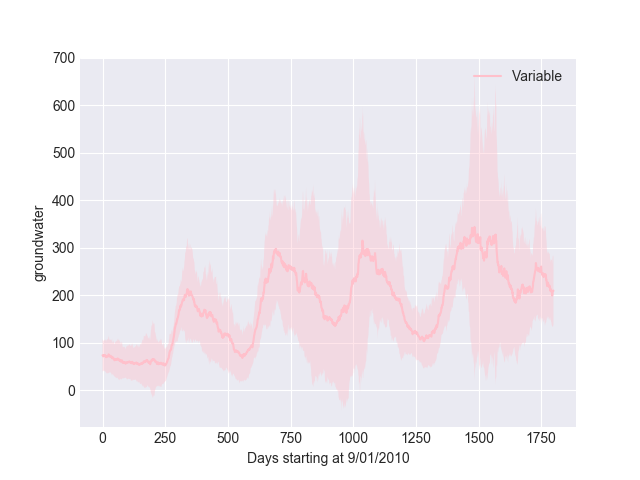
\includegraphics[width=.94\linewidth]{good_gw}
  \captionof{figure}{Perturbed groundwater}
  \label{fig:good_gw}
\end{minipage}
\end{figure}


\subsection{Continuous perturbation of streamflow and swe states}

Another method of decoupling the model's calibration process from its over-reliance on groundwater was through the direct perturbation of streamflow and swe states. This perturbation guaranteed that ensemble collapse was never fully realized.


\section{Small dataset}

To expedite the discovery of optimal initial values, errors, and minimum and maximum bounds for the complete dataset (see Table \ref{tab:t_param_min_max_initial}) the small dataset was run and compared with the ranges proposed by \cite{Seibert1997} and \cite{Wallner2013}.  The small dataset, which was comprised of 3 catchments around the Biterroot valley and consisted of one gauged catchment (henceforth referred to as catchment 241) and 2 ungauged catchments (catchments 244 and 248), was run over a period of 1800 days, or a little under 5 years. Simulations began in September so modeled snowfall accumulation could be corrected first, allowing accurate snow melts to inform streamflow runoff in the Spring and Summer. All parameters in the small dataset converged to a set of values within the first 250-500 days and did not deviate significantly from those chosen values for the remainder of the filtering process.

\subsection{Streamflow states and parameters}

\begin{figure}
\centering
\begin{minipage}{.33\textwidth}
  \centering
  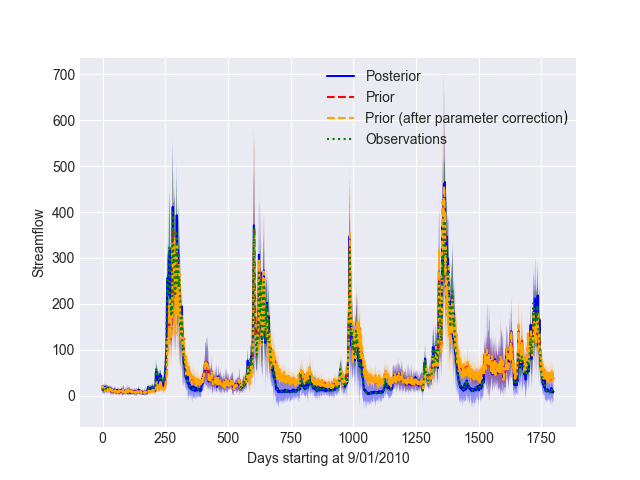
\includegraphics[width=.98\linewidth]{smallds_str_state_241}
  \label{fig:241st}
\end{minipage}%
\begin{minipage}{.33\textwidth}
  \centering
  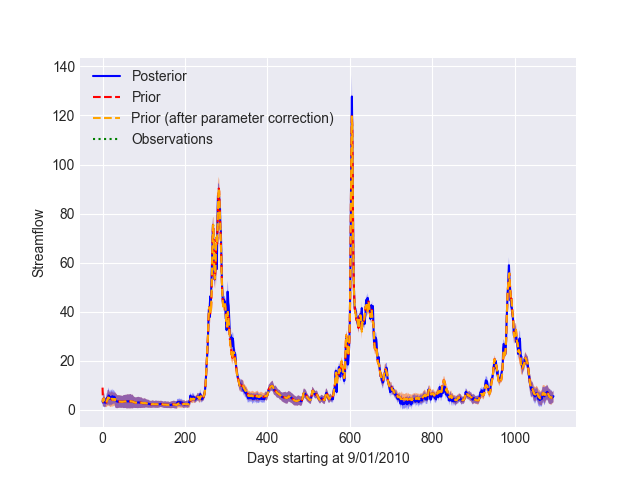
\includegraphics[width=.98\linewidth]{smallds_str_state_244}
  \label{fig:244st}
\end{minipage}
\begin{minipage}{.33\textwidth}
  \centering
  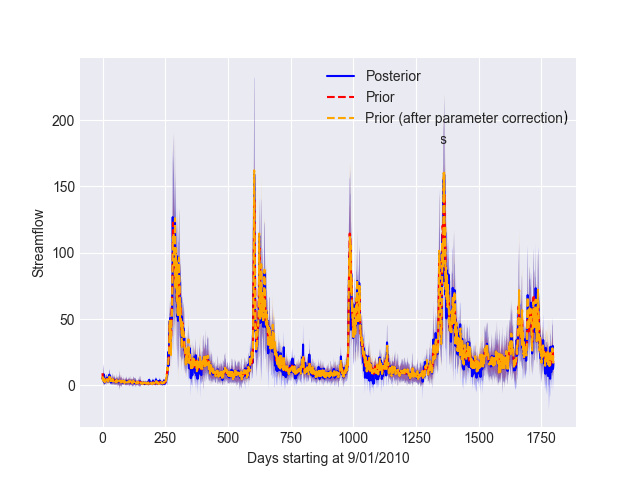
\includegraphics[width=.98\linewidth]{smallds_str_state_248}
  \label{fig:248st}
\end{minipage}
\captionof{figure}{Streamflow states for the 3 catchments}
\label{fig:str_state_small}
\end{figure}

All 3 posterior streamflow states (Figure \ref{fig:str_state_small}) snapped to the observations. The post-parameter correction streamflow (shown in yellow on the figures in \ref{fig:str_state_small}) also followed the observations in the Spring and Summer time periods. Notice the discrepancy between the post parameter correction state and posterior state seen in the first graph in Figure \ref{fig:str_state_small} during the Winter time periods. While state correction continuously tried to move streamflow down to a match the observed Winter state, parameters were not found that allowed streamflow to match the observed states. This result is connected to the behavior of the lower groundwater reservoir.

The lower groundwater reservoir in all three catchments  rose 100mm-200mm throughout the 1800 day filtering period (Figure \ref{fig:gw_small}). Throughout this time the filter's values for \texttt{ck2} and \texttt{perc}, two parameters that impact the buildup and dispersion of lower groundwater, remained unchanged. In this project, simulated groundwater was not compared to an observed state. Optimal groundwater behavior for the hydrologic model over long periods of time requires further research.

\begin{figure}
\centering
\begin{minipage}{.33\textwidth}
  \centering
  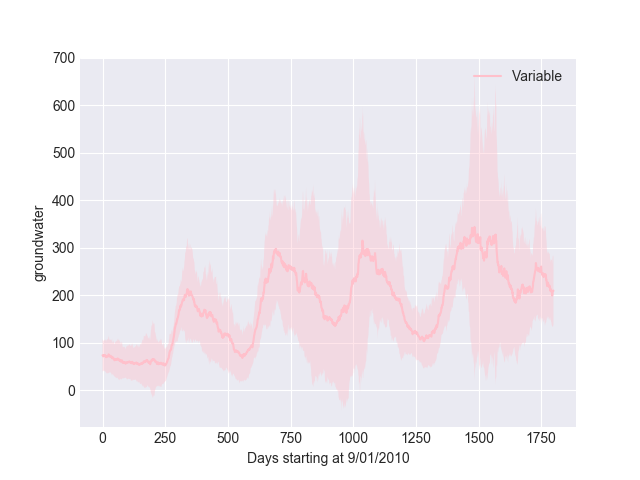
\includegraphics[width=.98\linewidth]{smallds_gw_state_241}
  \label{fig:241gw}
\end{minipage}%
\begin{minipage}{.33\textwidth}
  \centering
  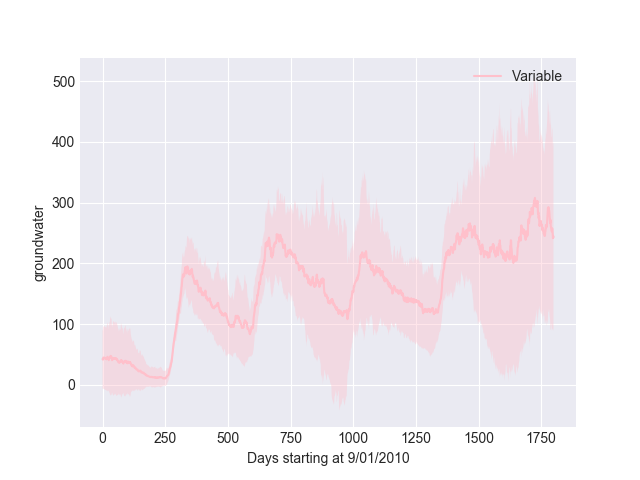
\includegraphics[width=.98\linewidth]{smallds_gw_state_244}
  \label{fig:244gw}
\end{minipage}
\begin{minipage}{.33\textwidth}
  \centering
  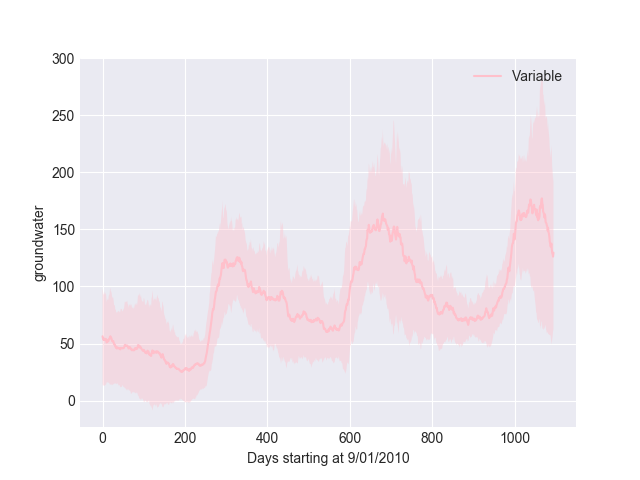
\includegraphics[width=.98\linewidth]{smallds_gw_state_248}
  \label{fig:248gw}
\end{minipage}
\captionof{figure}{Groundwaters for the 3 catchments}
\label{fig:gw_small}
\end{figure}

As seen in the plots in Figure \ref{fig:cks_small}, parameter ensembles converged to the ensemble mean within the first 200-400 days. All catchments also converged to similar values. Since this is a predictable outcome for the small geographic area the small dataset encompasses, the large dataset is a better indicator of the effects of the hierarchical component upon the spatial independence of spatially distributed catchments.

\begin{figure}[h]
    \centering
    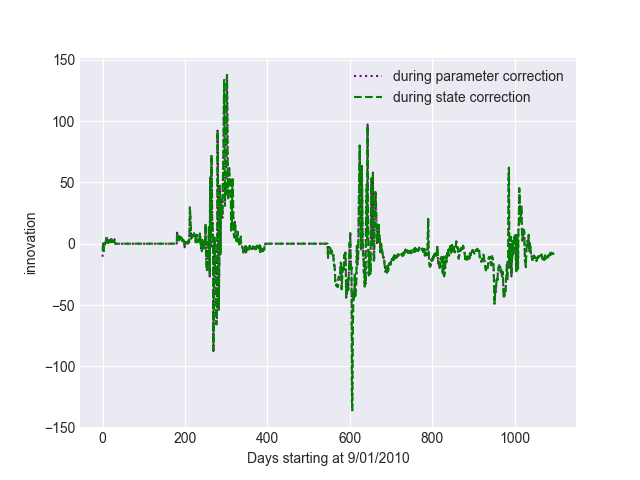
\includegraphics[width=0.5\textwidth]{str_innovation_small}
    \caption{Streamflow innovation (catchment 241)}
    \label{fig:str_innovation_small}
\end{figure}


\begin{figure}
\begin{tabular}{ccc}

\subcaptionbox{241:\texttt{ck0}\label{2}}{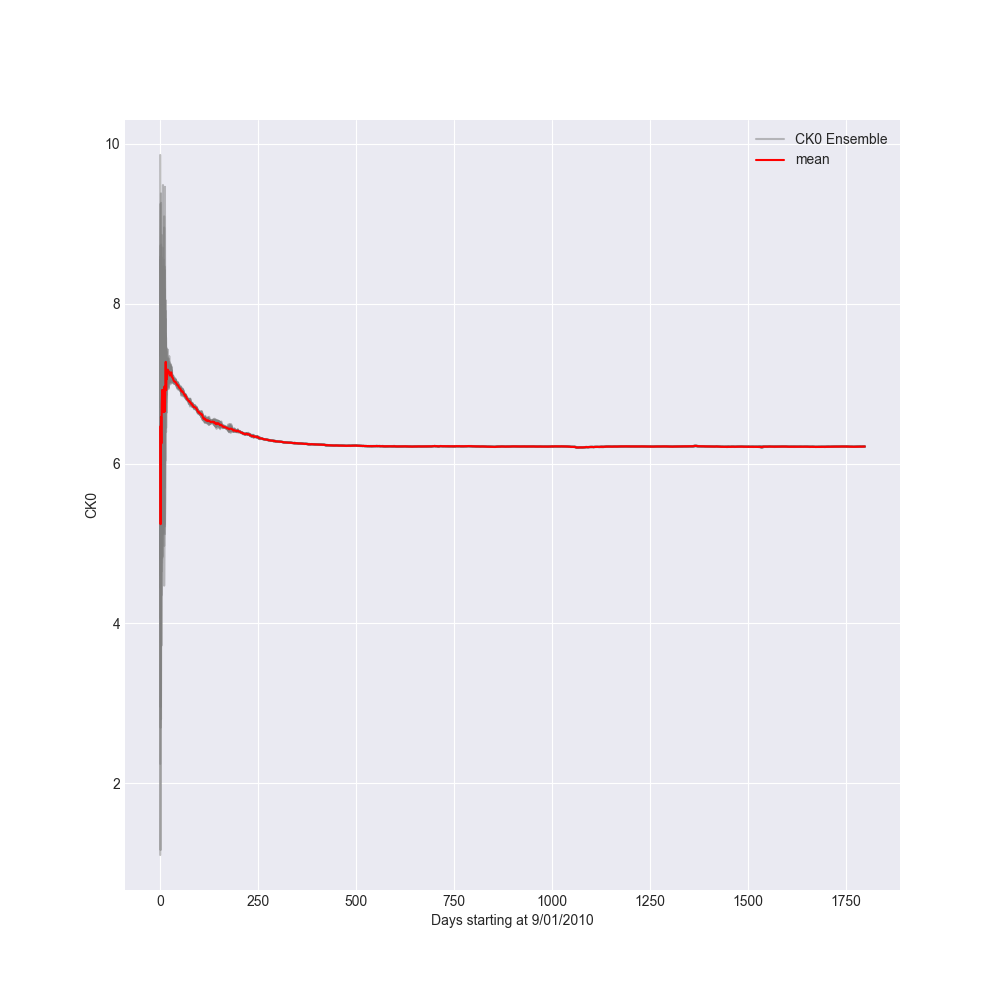
\includegraphics[width = .33\linewidth]{smallds_ck0_241}} &
\subcaptionbox{241:\texttt{ck1}\label{1}}{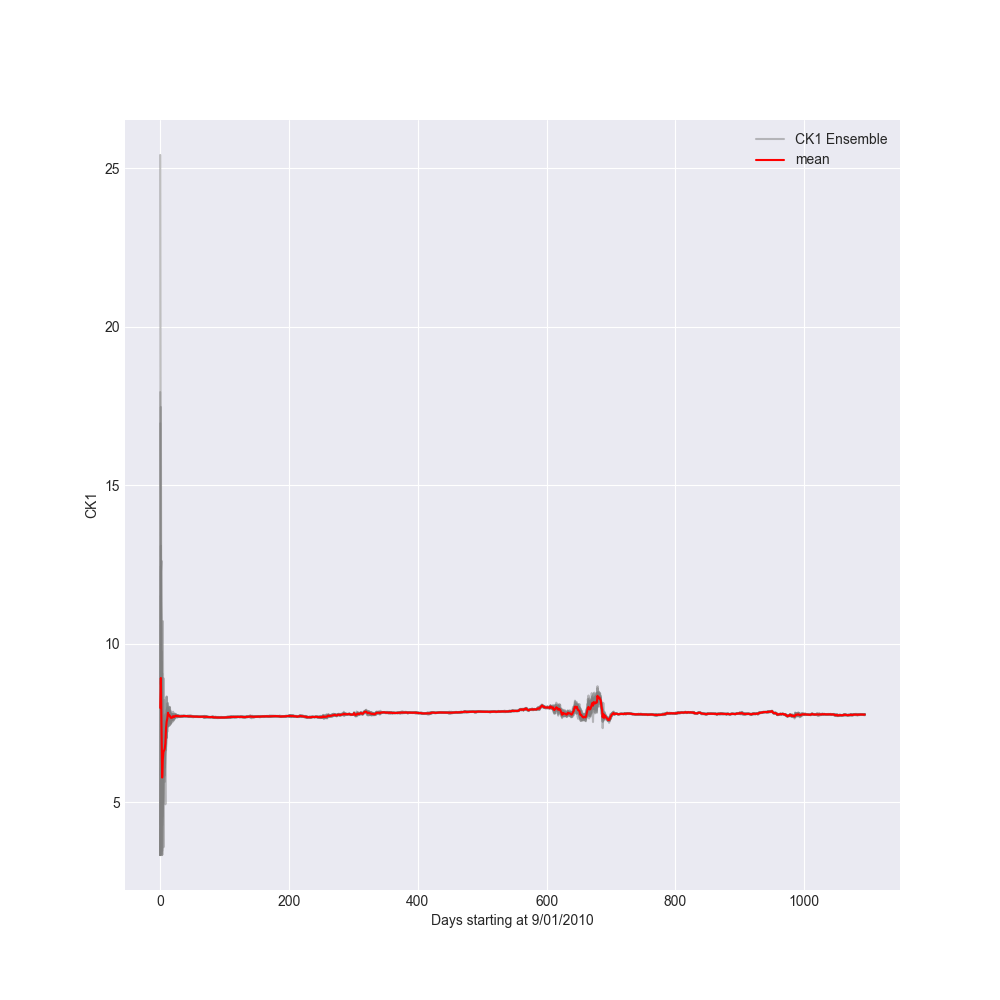
\includegraphics[width = .33\linewidth]{smallds_ck1_241}} &
\subcaptionbox{241:\texttt{ck2}\label{2}}{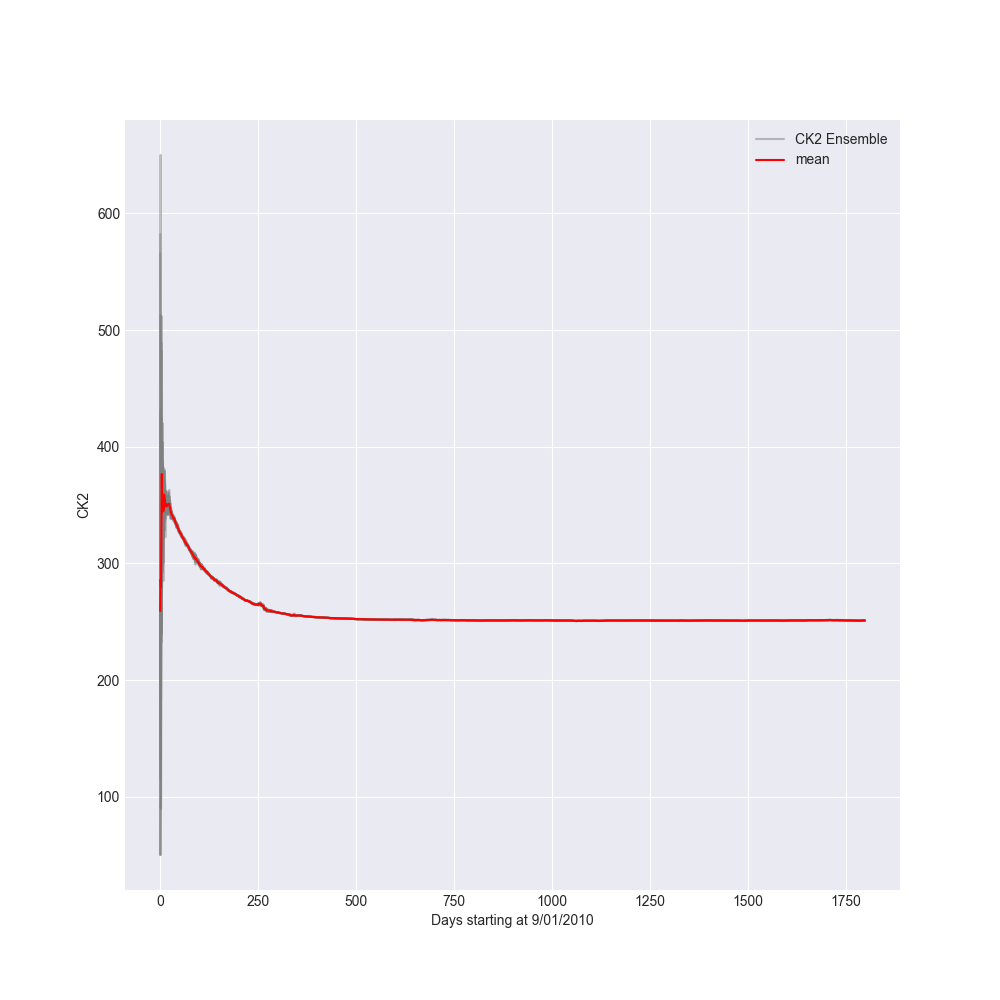
\includegraphics[width = .33\linewidth]{smallds_ck2_241}}\\
\subcaptionbox{244:\texttt{ck0}\label{2}}{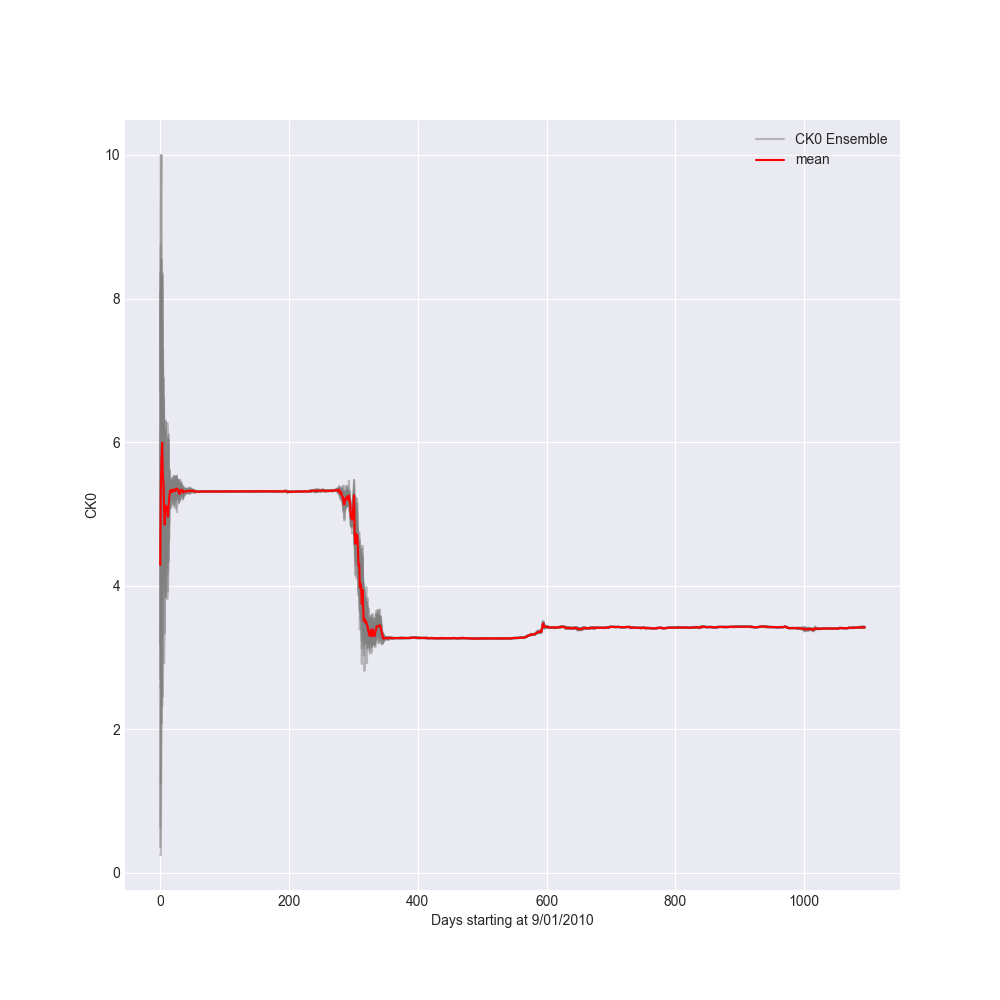
\includegraphics[width = .33\linewidth]{smallds_ck0_244}} &
\subcaptionbox{244:\texttt{ck1}\label{1}}{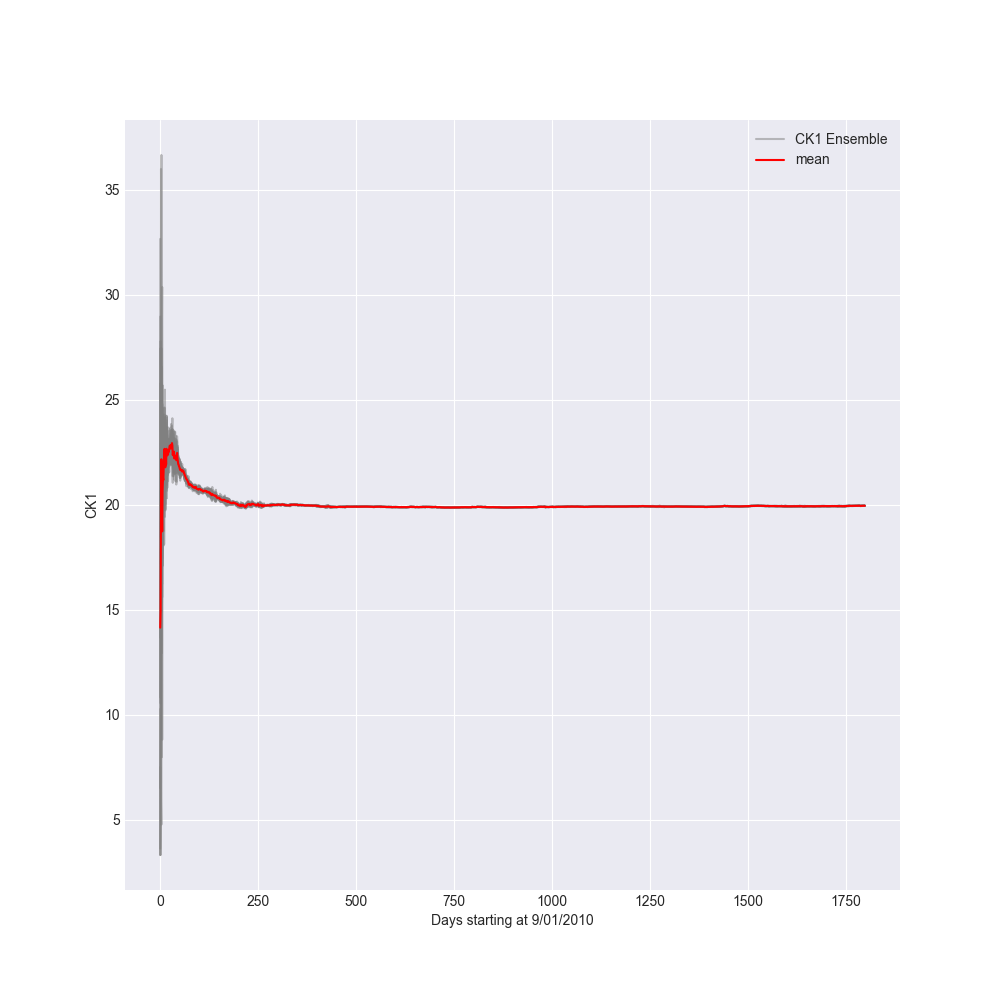
\includegraphics[width = .33\linewidth]{smallds_ck1_244}} &
\subcaptionbox{244:\texttt{ck2}\label{2}}{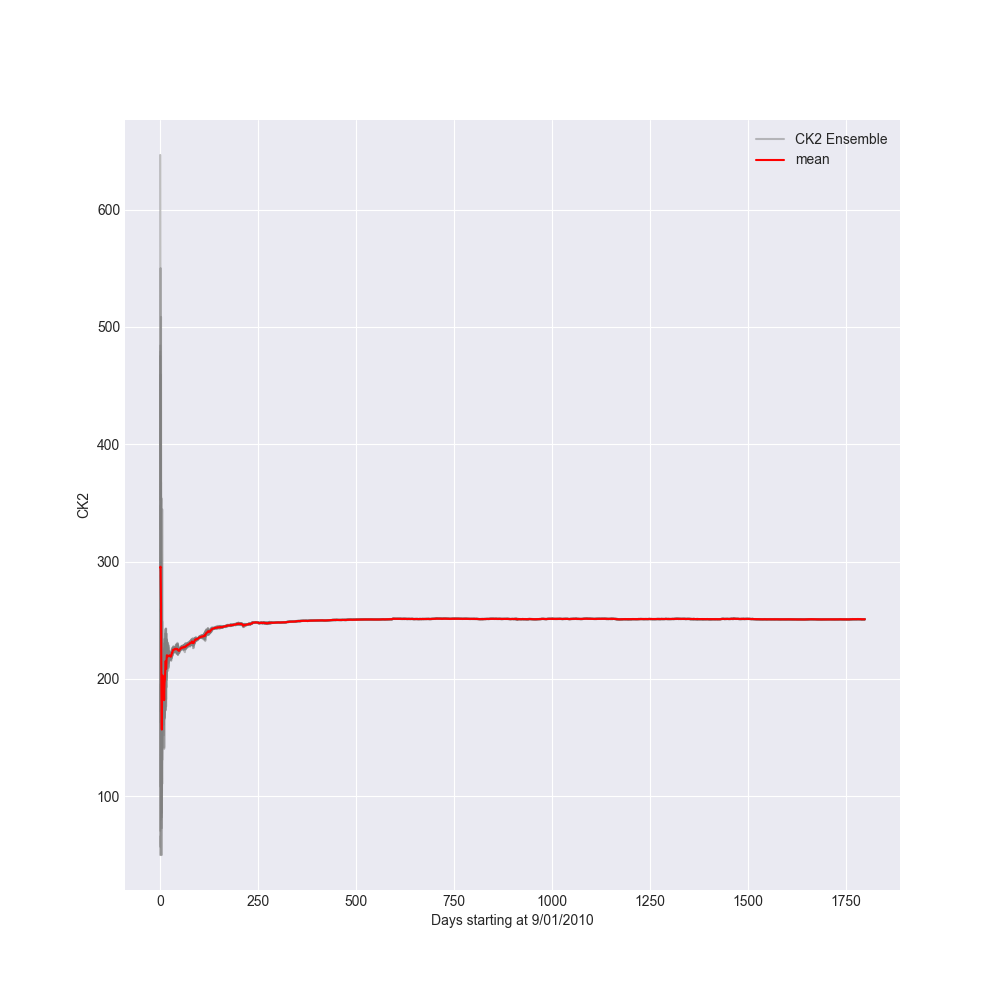
\includegraphics[width = .33\linewidth]{smallds_ck2_244}}\\
\subcaptionbox{248:\texttt{ck0}\label{2}}{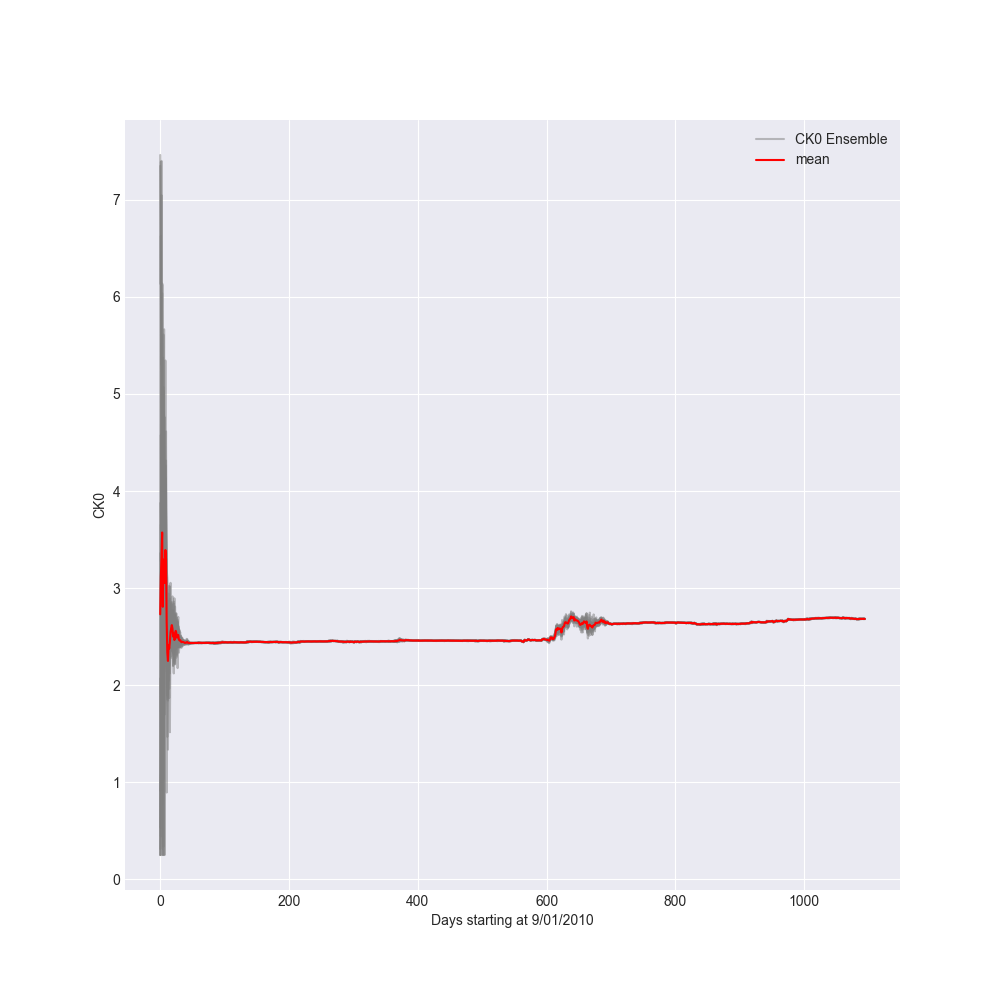
\includegraphics[width = .33\linewidth]{smallds_ck0_248}} &
\subcaptionbox{248:\texttt{ck1}\label{1}}{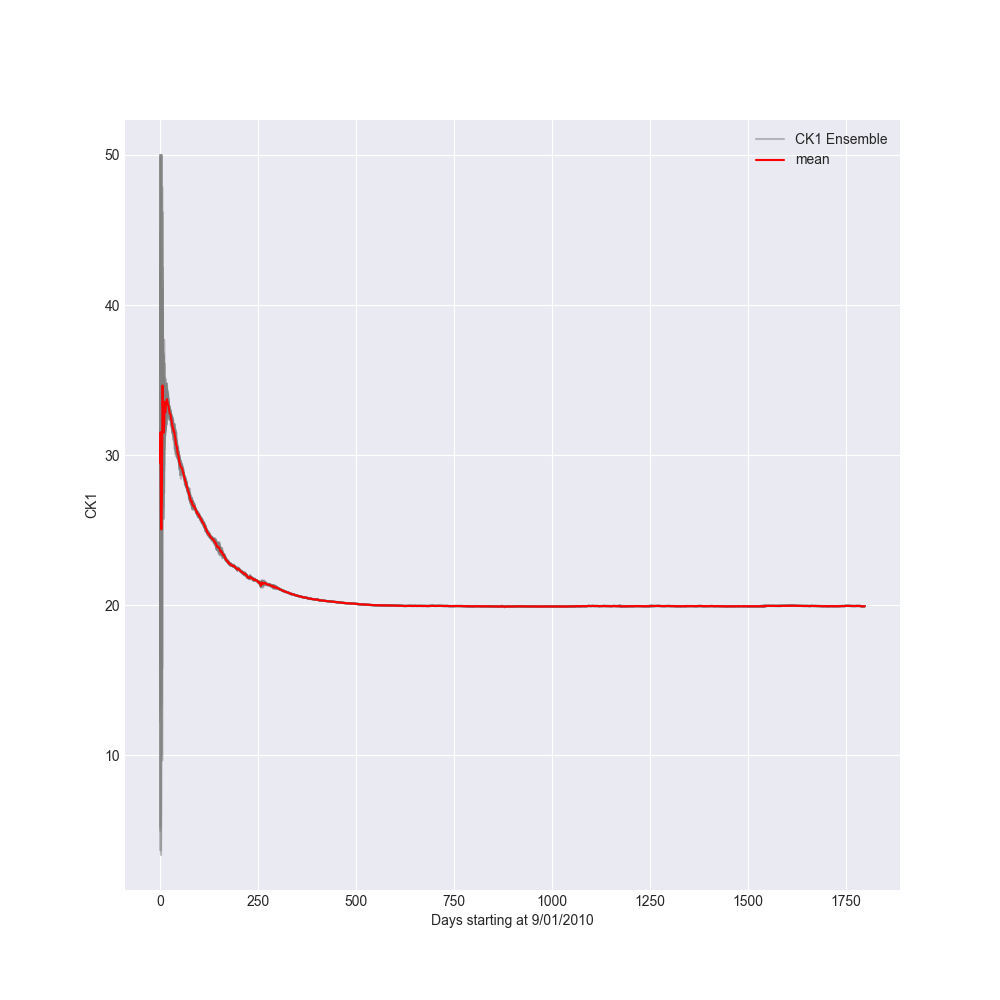
\includegraphics[width = .33\linewidth]{smallds_ck1_248}} &
\subcaptionbox{248:\texttt{ck2}\label{2}}{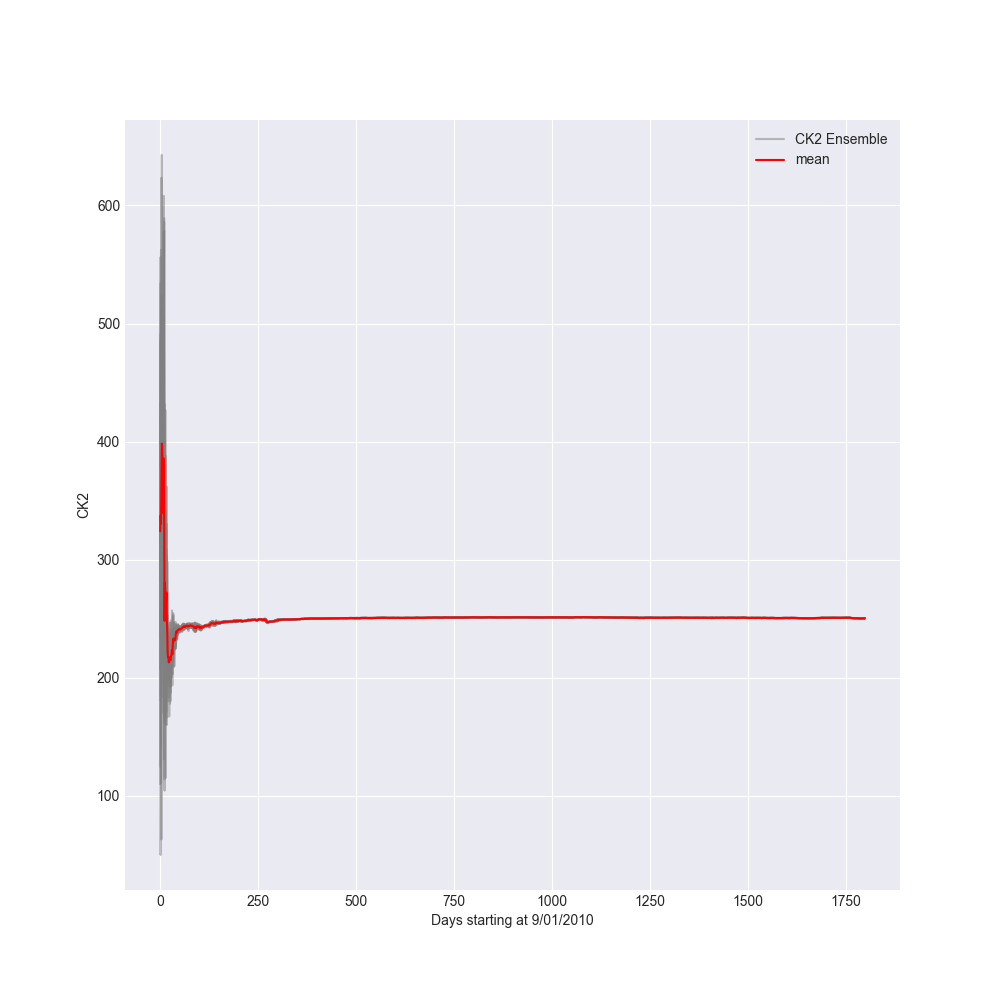
\includegraphics[width = .33\linewidth]{smallds_ck2_248}}

\end{tabular}
\label{fig:cks_small}
\captionof{figure}{Convergence of \texttt{ck} parameters for all 3 catchments}
\end{figure}

\begin{table}[]
\caption{Hyperparameters - parameter perturbations and min/max ranges} 
\begin{tabular}{llll}
Parameter ($\theta$) & $q$ & Min & Max \\ \hline
Degree Day Factor (\texttt{ddf})                 & .75mm$^\circ$C$^{-1}$d$^{-1}$ & 1mm$^\circ$C$^{-1}$d$^{-1}$ & 8mm$^\circ$C$^{-1}$d$^{-1}$ \\
Tempature Threshold (\texttt{thres})                & .5$^\circ$C & -2.5$^\circ$C & 2.5$^\circ$C \\
Potential Evapo-Transpiration (\texttt{aet\_lp})              & .15 & .3 & 1\\
Ponded water to soil storage (\texttt{soil\_beta})          & 1.75 & 1 & 6 \\
Soil compartment max capacity (\texttt{soil\_max\_wat})       & 40 & 50mm & 500mm \\
Immediate runoff (\texttt{ck0})       & 6d$^{-1}$ & .25d$^{-1}$ & 10d$^{-1}$ \\
Fast runoff (\texttt{ck1})      & 25d$^{-1}$ & 3.33d$^{-1}$ & 50d$^{-1}$\\
Groundwater runoff (\texttt{ck2})       & 350d$^{-1}$ & 50d$^{-1}$ & 650d$^{-1}$ \\
Groundwater water storage threshold (\texttt{hl1})       & 25mm & 0mm & 50mm \\
Groundwater peculation (\texttt{perc})       & 1.5d & 3d & 50d \\
Wave celerity (\texttt{K})         & 82400 & 81576 & 84872 \\
Wave dispersion (\texttt{e})       & .35 & .25 & .4 \\
\end{tabular}
\label{tab:t_param_min_max_initial}
\end{table}

\subsection{Snow-water equivalent states and parameters}

\begin{figure}
\centering
\begin{minipage}{.33\textwidth}
  \centering
  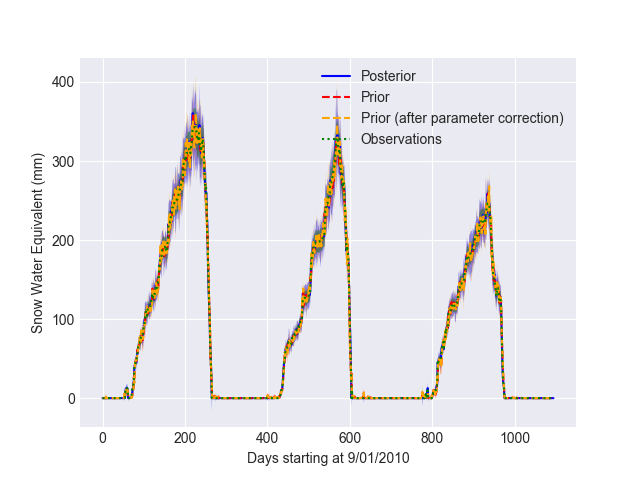
\includegraphics[width=.98\linewidth]{smallds_swe_state_241}
  \label{fig:241swe}
\end{minipage}%
\begin{minipage}{.33\textwidth}
  \centering
  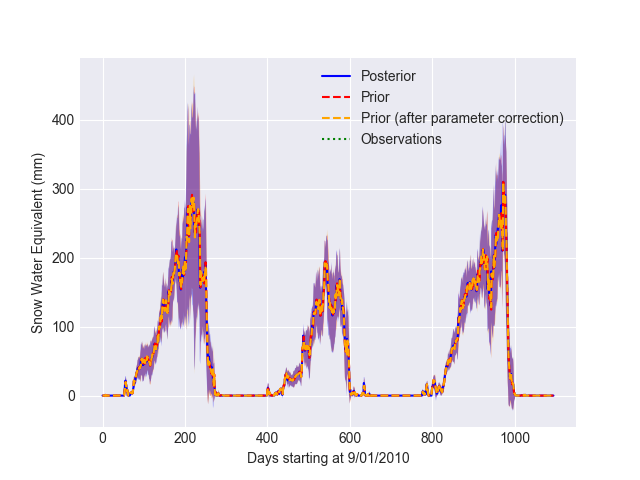
\includegraphics[width=.98\linewidth]{smallds_swe_state_244}
  \label{fig:244swe}
\end{minipage}
\begin{minipage}{.33\textwidth}
  \centering
  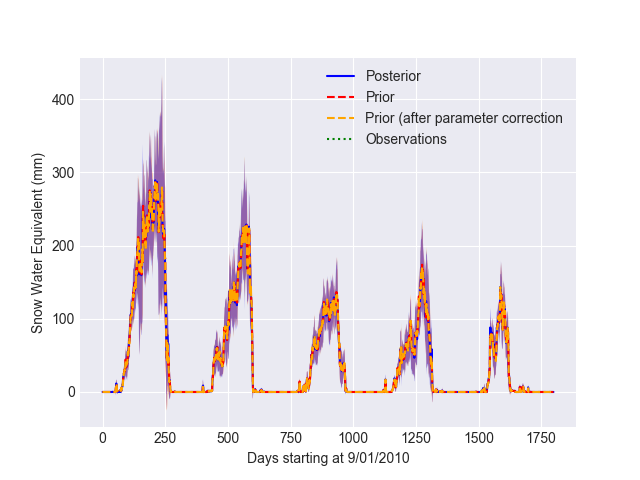
\includegraphics[width=.98\linewidth]{smallds_swe_state_248}
  \label{fig:248swe}
\end{minipage}
\captionof{figure}{Snow-water equivalent states for the 3 catchments}
\label{fig:swe_state_small}
\end{figure}


\begin{figure}[h]
    \centering
    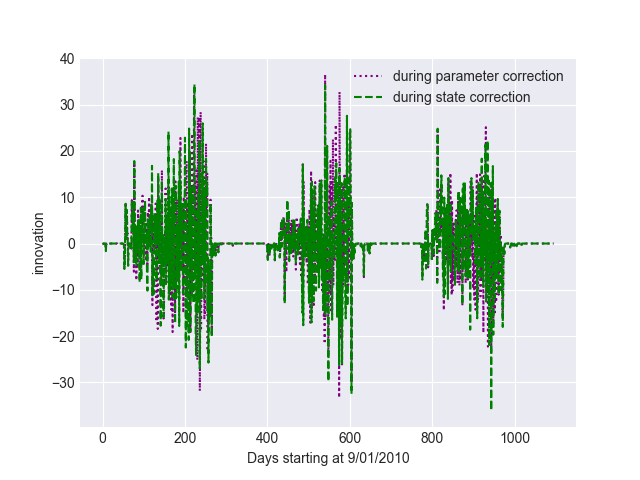
\includegraphics[width=0.5\textwidth]{swe_innovation_small}
    \caption{SWE innovation (catchment 241)}
    \label{fig:swe_innovation_small}
\end{figure}

Snow-water equivalent states and parameters behaved similarly to their streamflow counterparts. Snow-water equivalent states (Figure \ref{fig:swe_state_small}) snapped to the observations quickly. Snow-water equivalent innovation (Figure \ref{fig:swe_innovation_small}) is much less biased then streamflow innovation (Figure \ref{fig:str_innovation_small}). Snow-water equivalent parameters behaved similarly to their streamflow counterparts. All ensembles and catchments converged to a very similar value within the first 200-400 timesteps (Figure \ref{fig:swe_params_small}.)



\begin{figure}
\begin{tabular}{cc}

\subcaptionbox{241:\texttt{ck0}\label{2}}{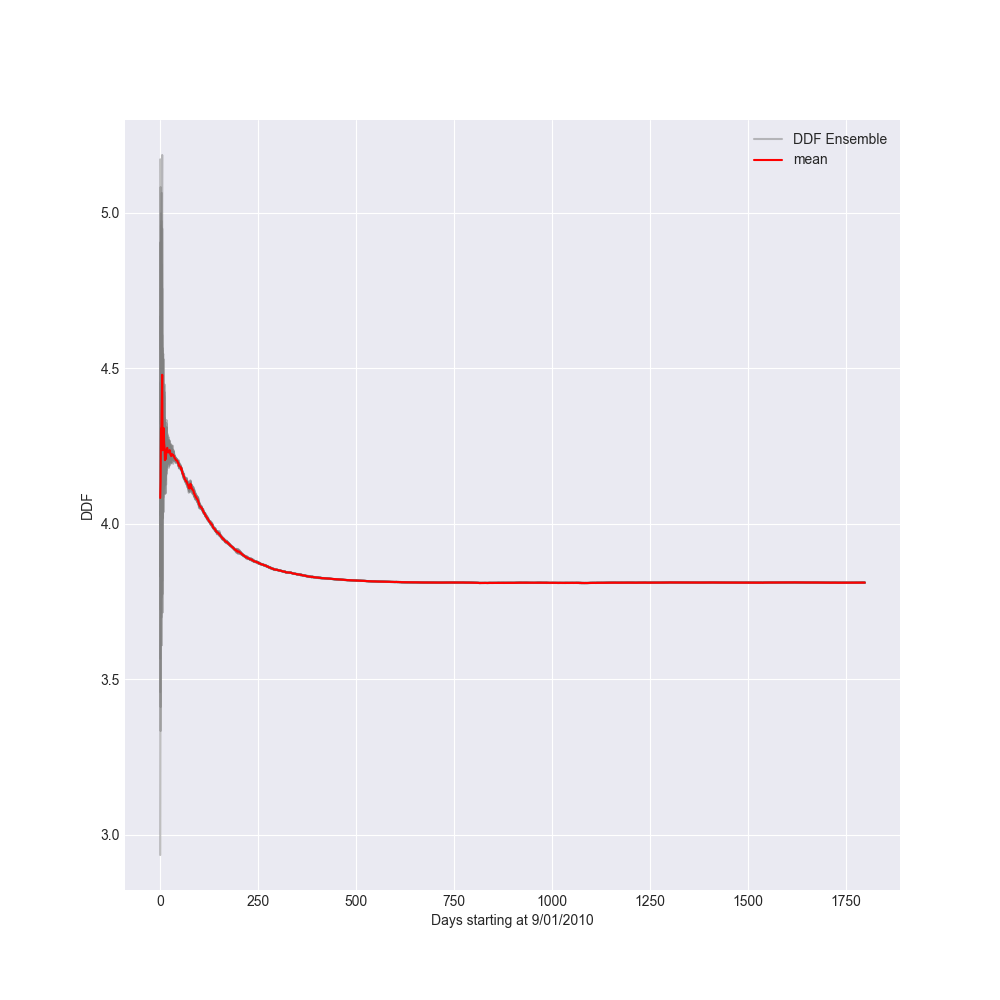
\includegraphics[width = .48\linewidth]{smallds_ddf_241}} &
\subcaptionbox{241:\texttt{ck2}\label{2}}{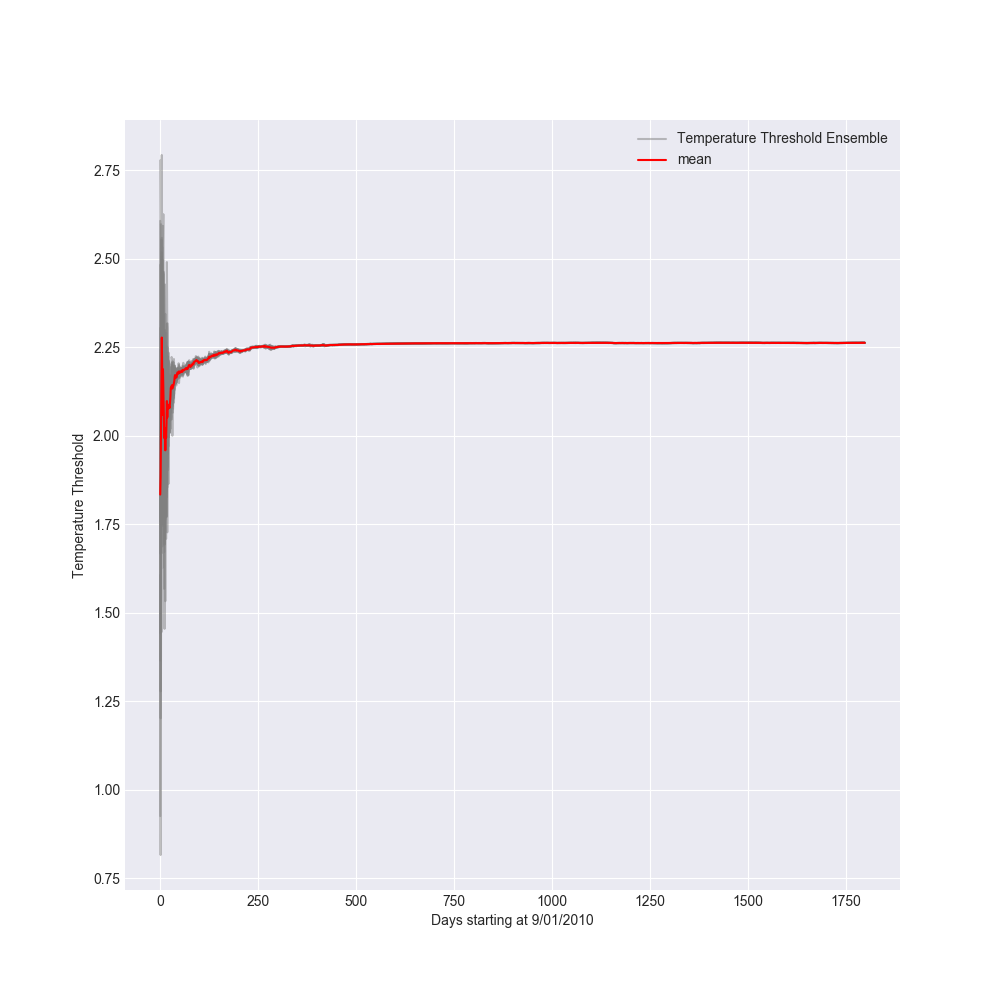
\includegraphics[width = .48\linewidth]{smallds_pp_241}}\\
\subcaptionbox{244:\texttt{ck0}\label{2}}{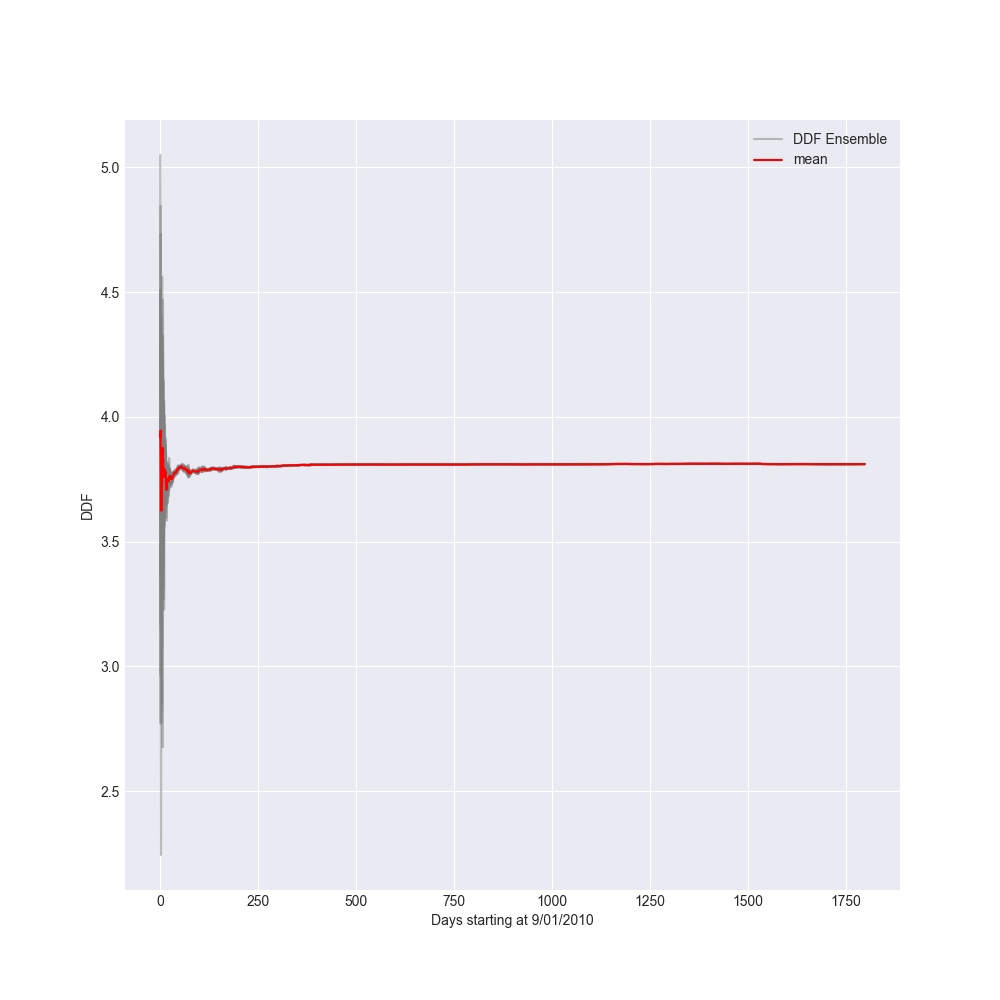
\includegraphics[width = .48\linewidth]{smallds_ddf_244}} &
\subcaptionbox{244:\texttt{ck2}\label{2}}{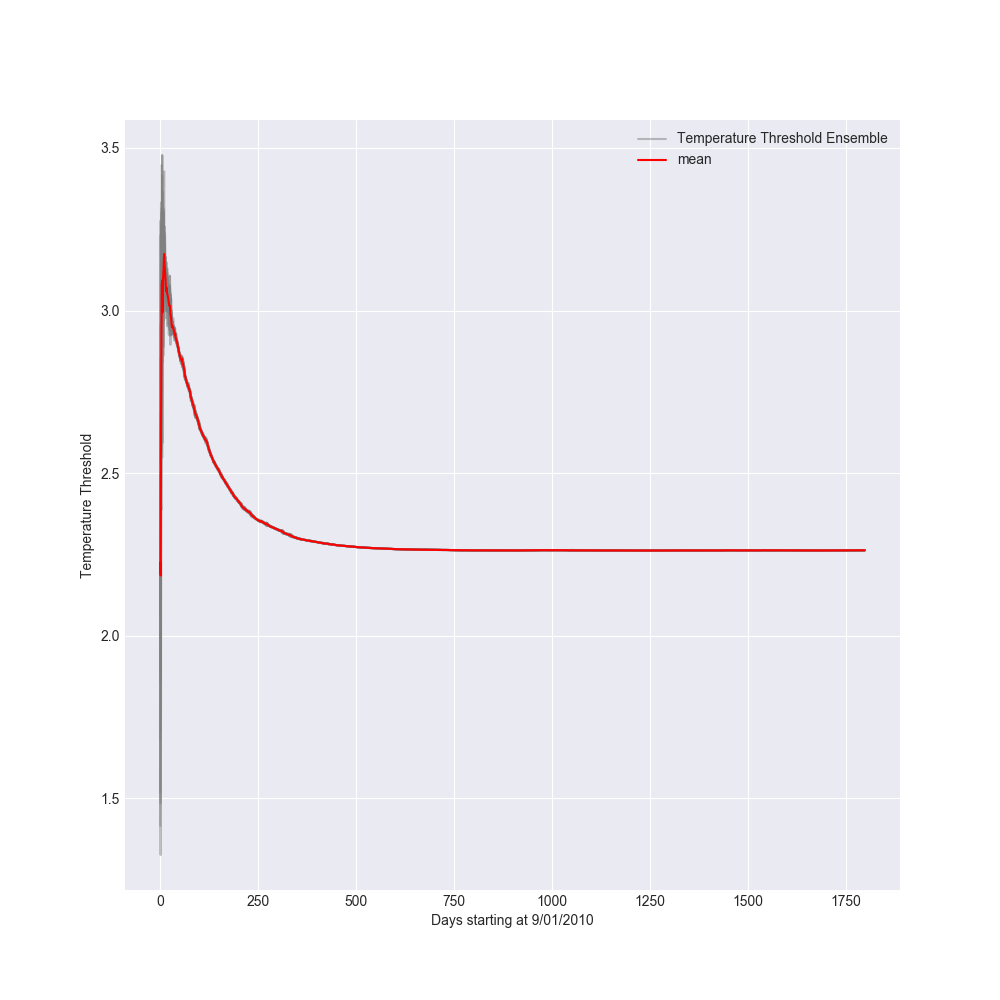
\includegraphics[width = .48\linewidth]{smallds_pp_244}}\\
\subcaptionbox{248:\texttt{ck0}\label{2}}{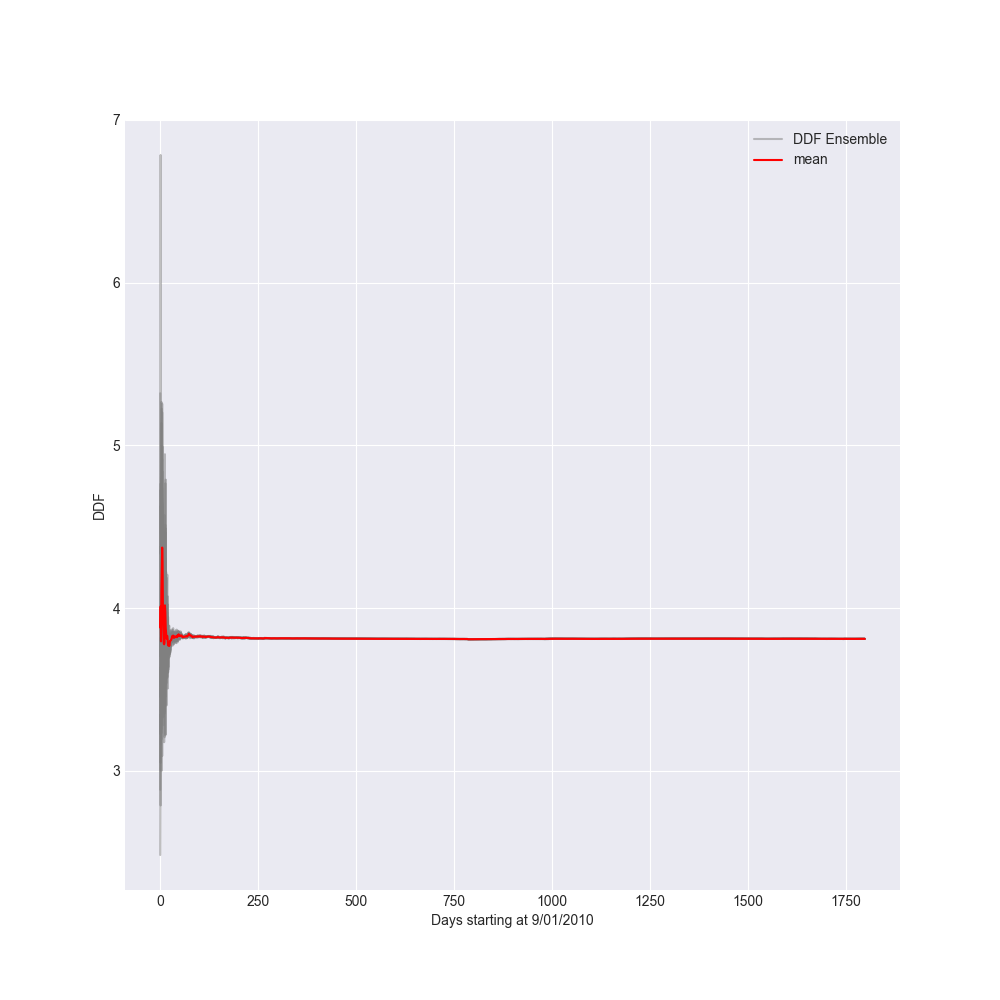
\includegraphics[width = .48\linewidth]{smallds_ddf_248}} &
\subcaptionbox{248:\texttt{ck1}\label{1}}{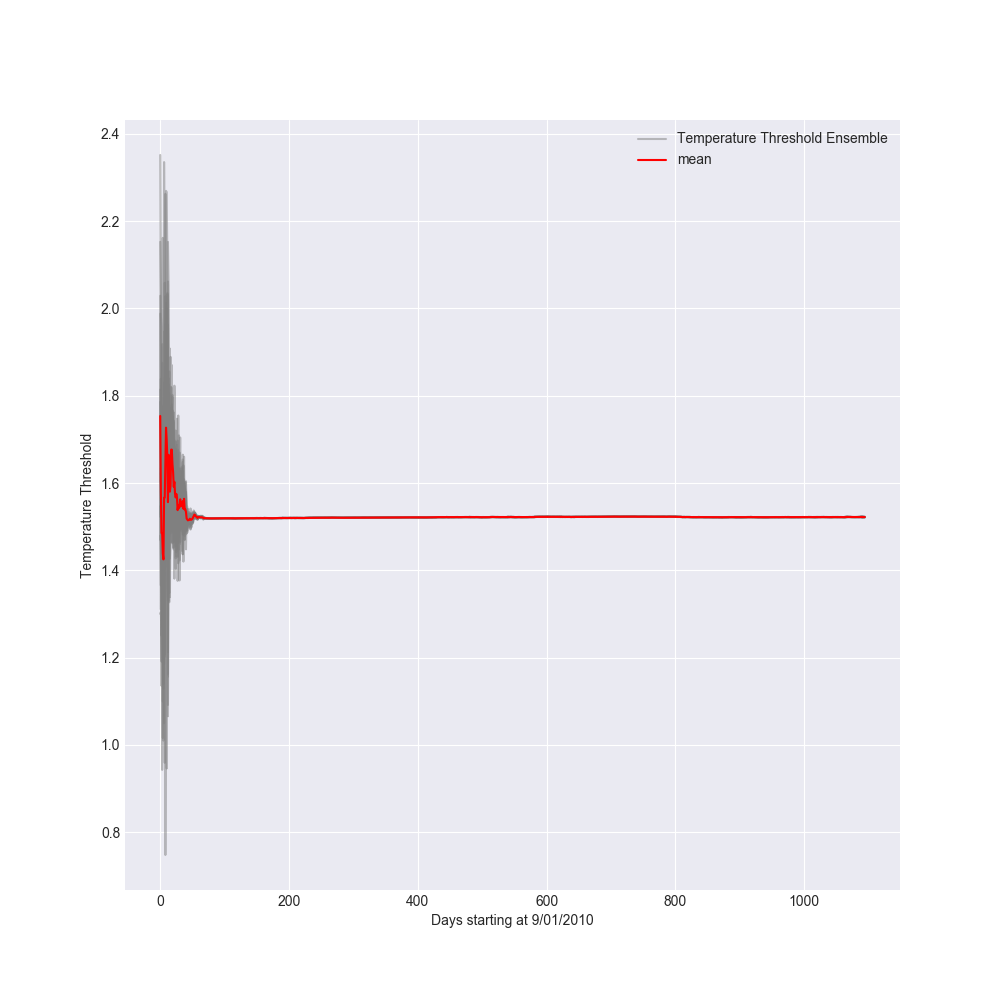
\includegraphics[width = .48\linewidth]{smallds_pp_248}}

\end{tabular}
\label{fig:str_params_small}
\captionof{figure}{Convergence of \texttt{ck} parameters for all 3 catchments}
\end{figure}

\begin{figure}
\begin{tabular}{cc}

\subcaptionbox{All catchments:\texttt{ddf}\label{group17swe_ddf_small}}{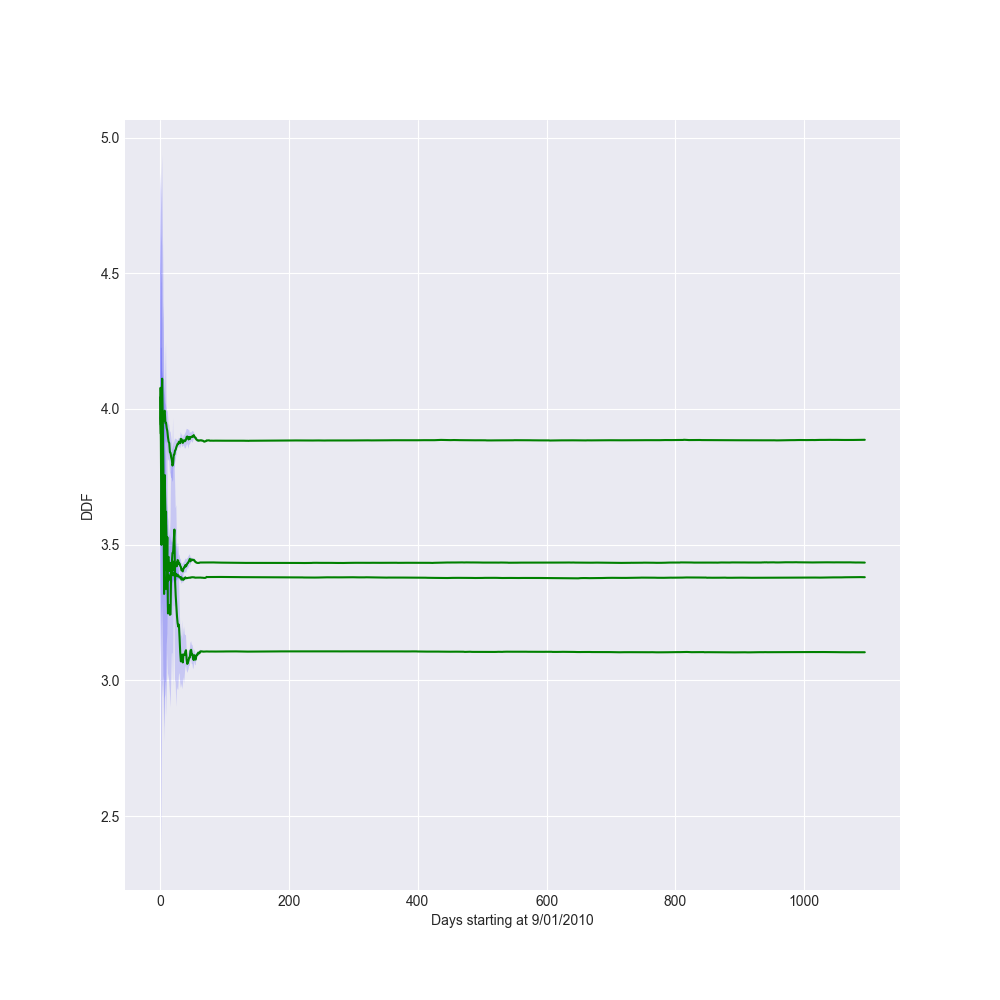
\includegraphics[width = .48\linewidth]{group17swe_ddf_small}} &
\subcaptionbox{All catchments:\texttt{pp}\label{group17swe_pp_small}}{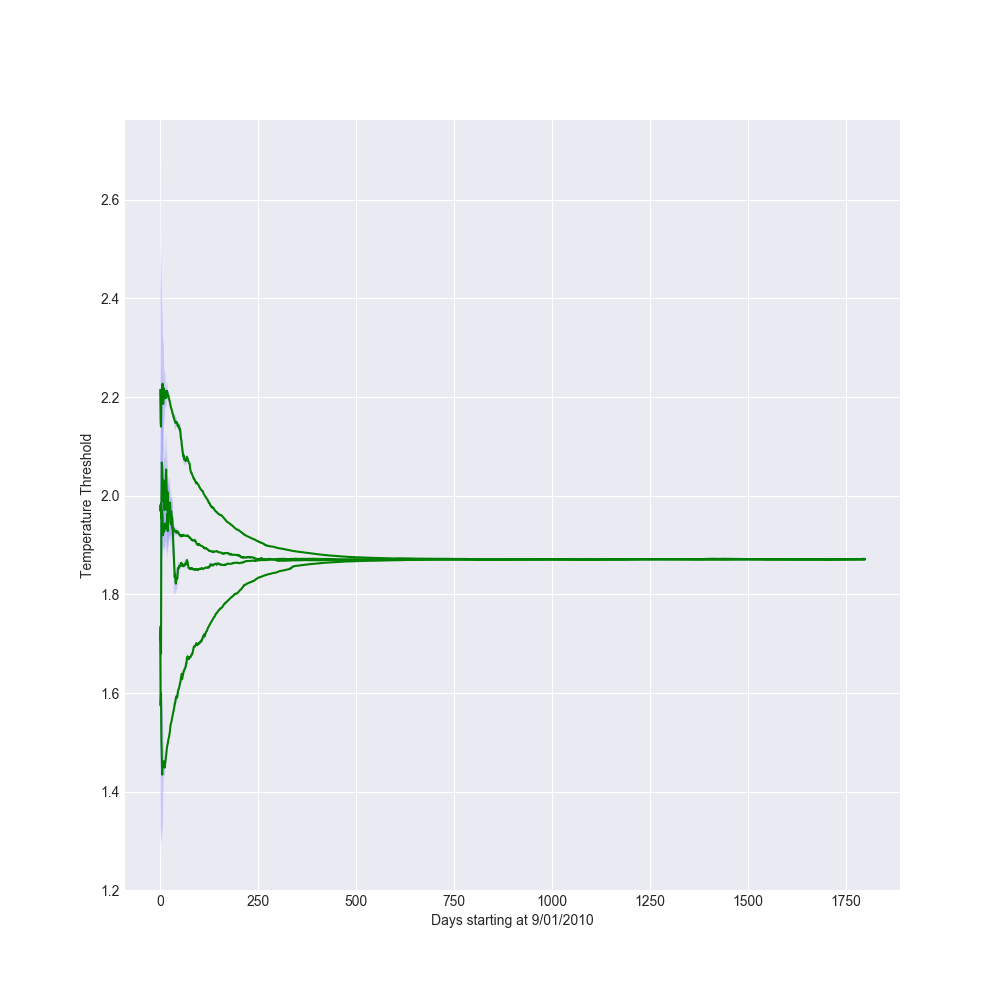
\includegraphics[width = .48\linewidth]{group17swe_pp_small}}
\end{tabular}
\label{fig:swe_params_small}
\captionof{figure}{All SWE parameters throughout the small dataset converged to a similar value. \texttt{a} blending value = .009}
\end{figure}


\section{Complete Dataset}

After workable initial values, errors, and boundaries and had been selected the complete dataset was calibarated. Calibration of the complete dataset was computationally expensive and a balance had to be struck between ensemble size, time run, and data collected per timestep. For these results a full year (365 days) was run with 125 ensemble members. Running periods larger then one year came at the price of reducing the ensemble members, which led to unstable and unusable posterior corrections (Figure \ref{fig:327str_1yr2yr_compare}). Running the DSHKEnKF on the large dataset produced mixed results that point to both strengths in the hierarchical design and further research opportunities.

\subsection{Streamflow states and parameters}

Streamflow calibration on the large dataset proved to be a difficult process. While the posterior state vector matched the observations, innovation was heavily biased and both the prior and post-parameter correction prior had trouble locking onto parameters during the Summer months, resulting in an unstable prior and biased innovation (Figure \ref{fig:str_state_296}.) This erratic behavior was more pronounced before it was reduced by the changes referenced in \autoref{sec:perturbation_of_states}. Unfortunately, these techniques could not be utilized to entirely balance the innovation since excessive state noise resulted in overly weak and unreliable parameter correction.


\begin{figure}
\centering
\begin{minipage}{.48\textwidth}
  \centering
  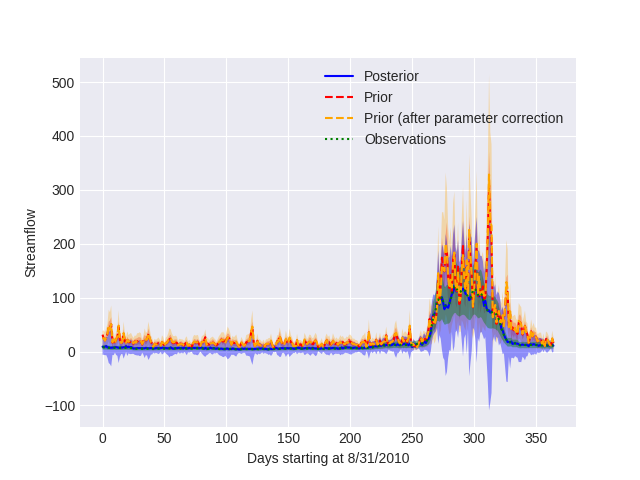
\includegraphics[width=.98\linewidth]{ds_str_state_296}
  \label{fig:296str}
\end{minipage}%
\begin{minipage}{.48\textwidth}
  \centering
  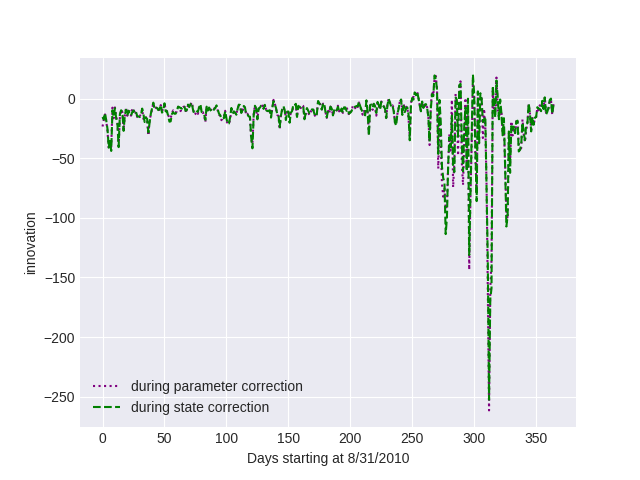
\includegraphics[width=.98\linewidth]{ds_str_state_296_innovation}
  \label{fig:296strinnovation}
\end{minipage}
\captionof{figure}{A gauged streamflow state and its innovation}
\label{fig:str_state_296}
\end{figure}


\subsection{Snow-water equivalent states and parameters}

Snow-water equivalent calibration on the large dataset was similar to the calibration of the small dataset and is a better demonstration of the successful calibration of a large-scale model component then streamflow calibration.

While \texttt{ddf} and \texttt{pp} were not run in a sufficient amount of time to stabilize to a value due to the aforementioned computational limitations, all catchments (Figure \ref{fig:swe_params}) are seen behaving in a similar fashion to their small dataset counterparts (Figure \ref{fig:swe_params_small}.)

\begin{figure}
\centering
\begin{minipage}{.33\textwidth}
  \centering
  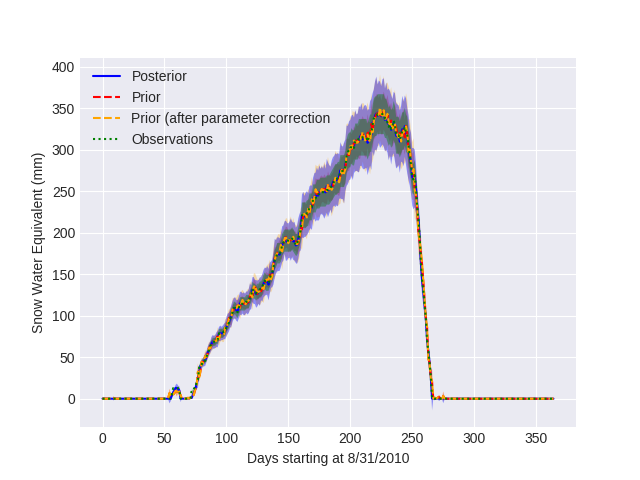
\includegraphics[width=.98\linewidth]{ds_swe_state_241}
  \label{fig:ds_swe_state_241}
\end{minipage}%
\begin{minipage}{.33\textwidth}
  \centering
  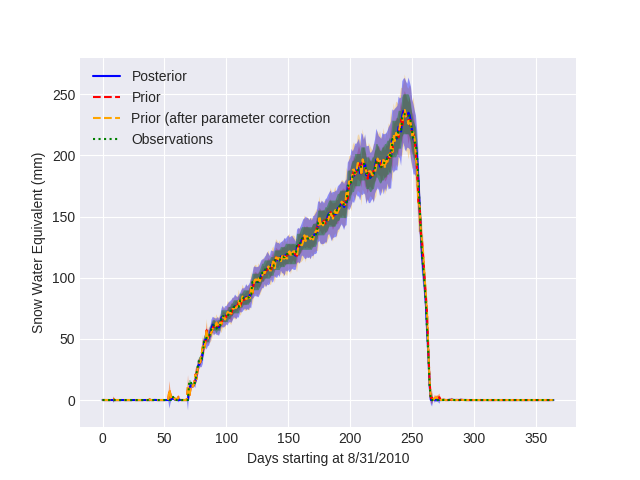
\includegraphics[width=.98\linewidth]{ds_swe_state_302}
  \label{fig:ds_swe_state_302}
\end{minipage}
\begin{minipage}{.33\textwidth}
  \centering
  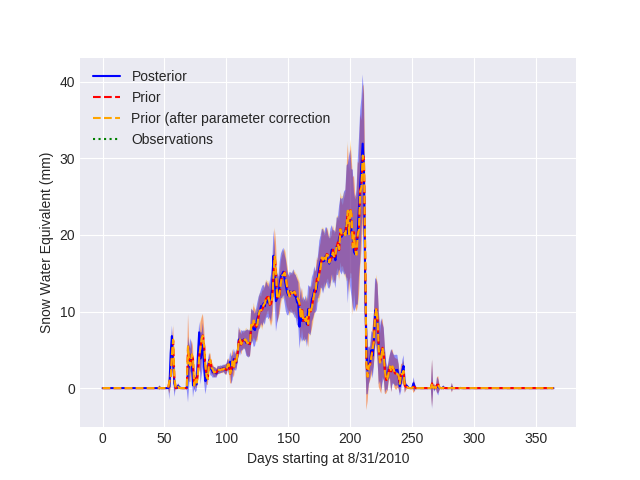
\includegraphics[width=.98\linewidth]{ds_swe_state_305}
  \label{fig:ds_swe_state_305}
\end{minipage}
\captionof{figure}{Snow-water equivalent states for 3 catchments: 241 (gauged), 302 (gauged), and 305 (ungauged)}
\label{fig:swe_state}
\end{figure}

\begin{figure}
\centering
\begin{minipage}{.48\textwidth}
  \centering
  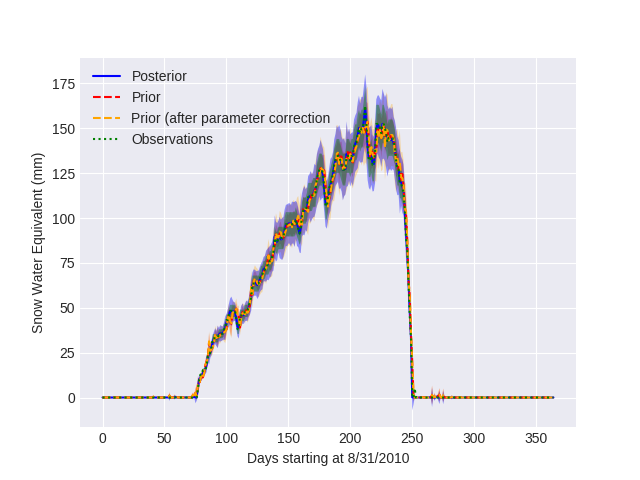
\includegraphics[width=.98\linewidth]{ds_swe_state_193}
  \label{fig:ds_swe_state_193}
\end{minipage}%
\begin{minipage}{.48\textwidth}
  \centering
  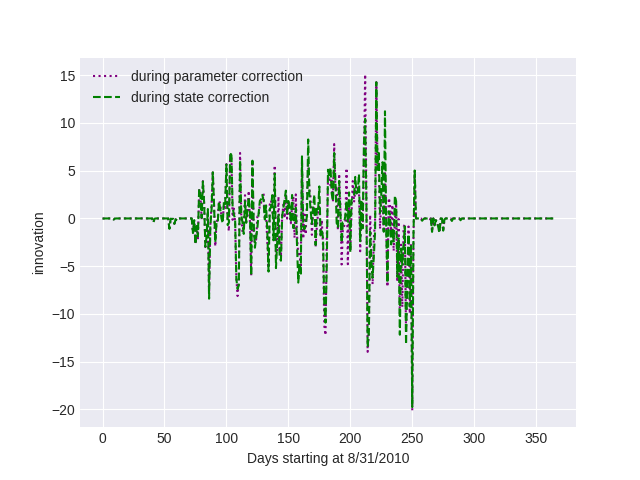
\includegraphics[width=.98\linewidth]{ds_swe_state_193_innovation}
  \label{fig:ds_swe_state_193_innovation}
\end{minipage}
\captionof{figure}{A gauged swe state and its innovation (catchment 193)}
\label{fig:swestate193}
\end{figure}

\begin{figure}
\centering
\begin{minipage}{.48\textwidth}
  \centering
  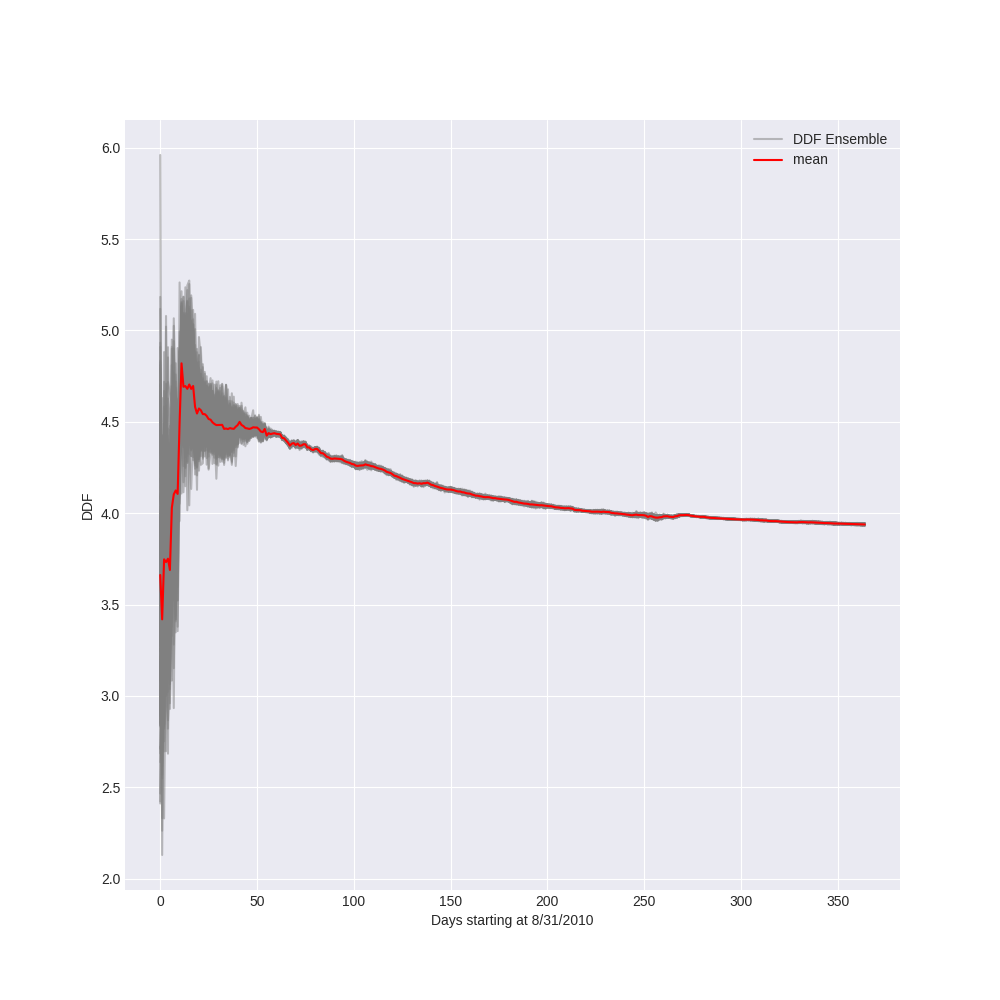
\includegraphics[width=.999\linewidth]{ds_ddf_193}
  \label{fig:ds_ddf_193}
\end{minipage}%
\begin{minipage}{.48\textwidth}
  \centering
  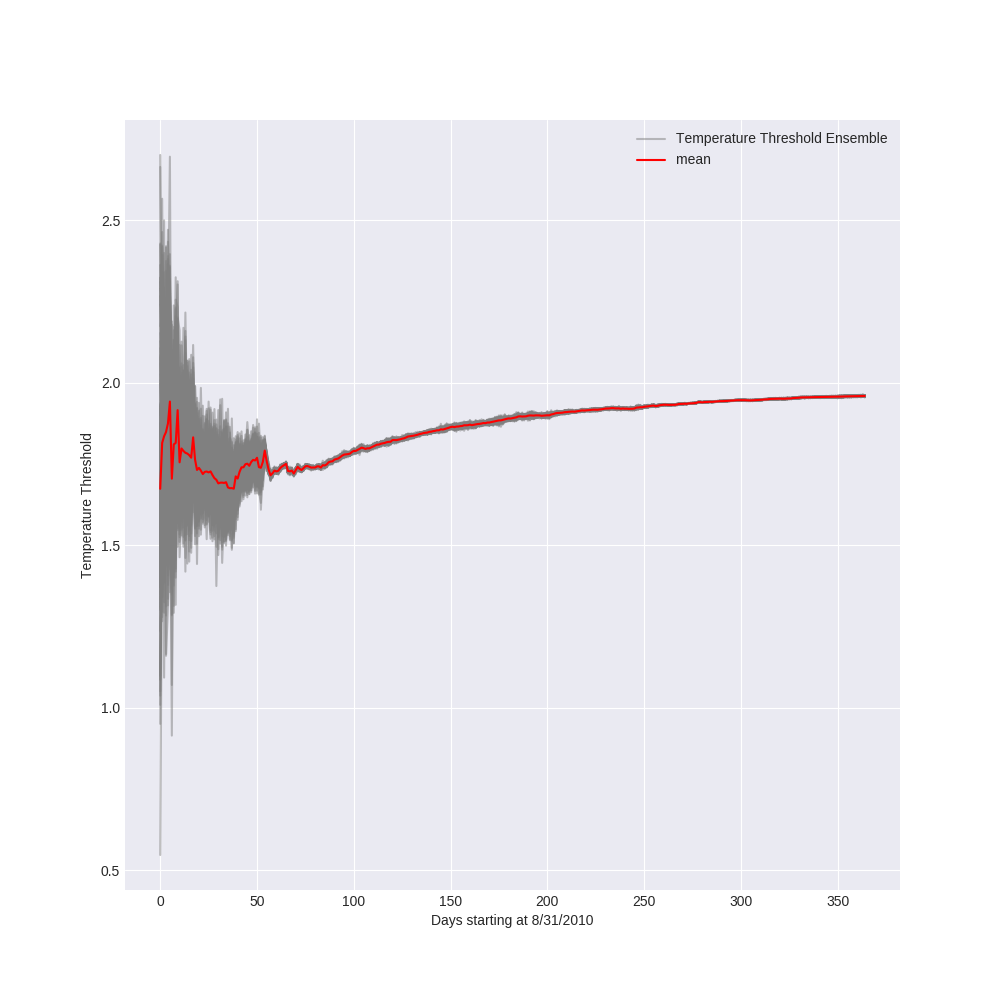
\includegraphics[width=.999\linewidth]{ds_pp_193}
  \label{fig:ds_pp_193}
\end{minipage}
\captionof{figure}{ddf and temperature threshold - catchment 193}
\label{fig:sweparams193}
\end{figure}

\begin{figure}
\begin{tabular}{cc}

\subcaptionbox{Hierarchical Group 1:\texttt{ddf}\label{2}}{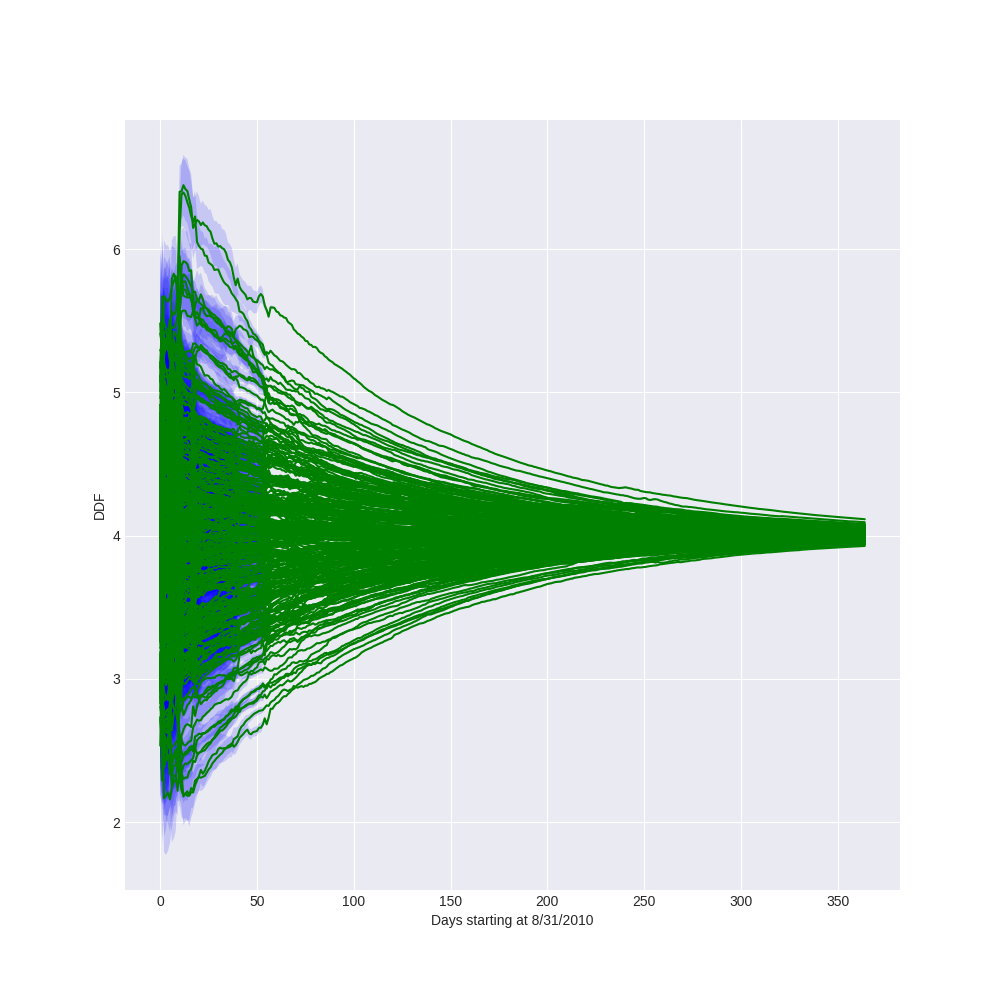
\includegraphics[width = .48\linewidth]{group10swe_ddf}} &
\subcaptionbox{Hierarchical Group 1:\texttt{pp}\label{2}}{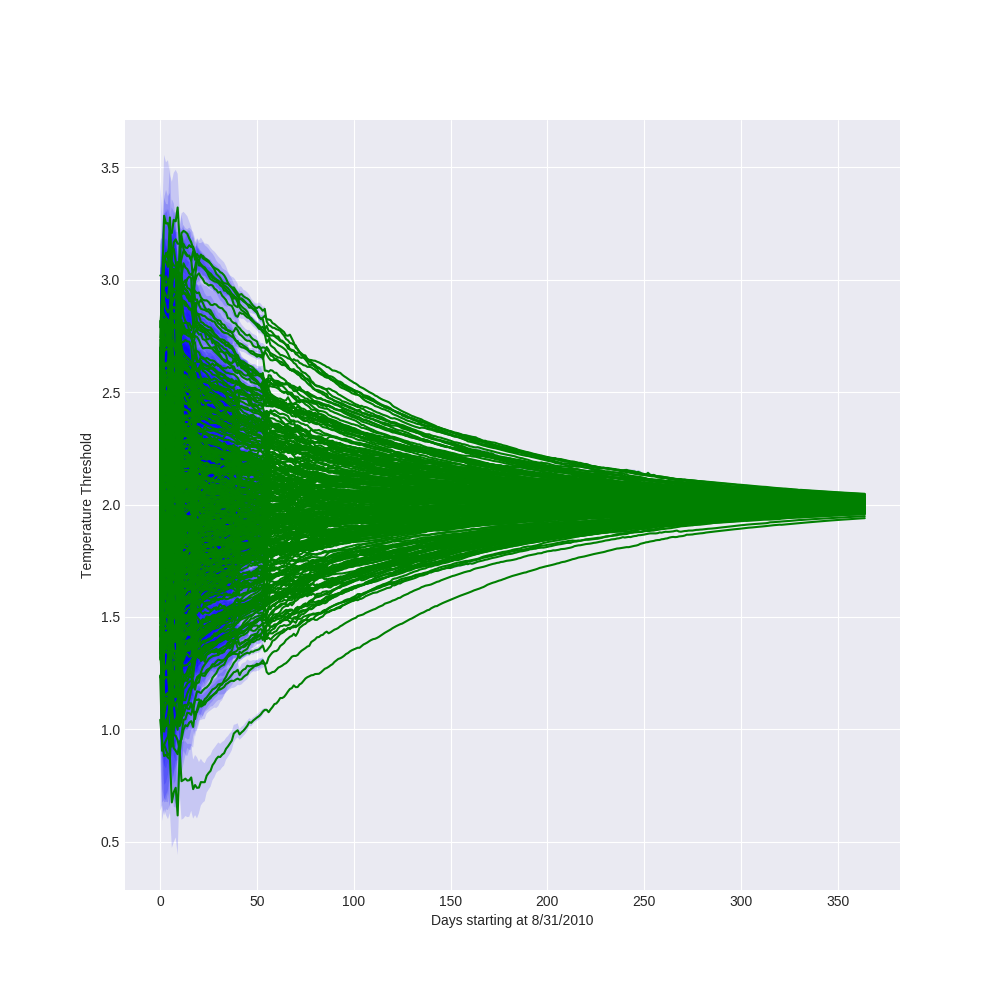
\includegraphics[width = .48\linewidth]{group10swe_pp}}\\
\subcaptionbox{Hierarchical Group 2:\texttt{ddf}\label{2}}{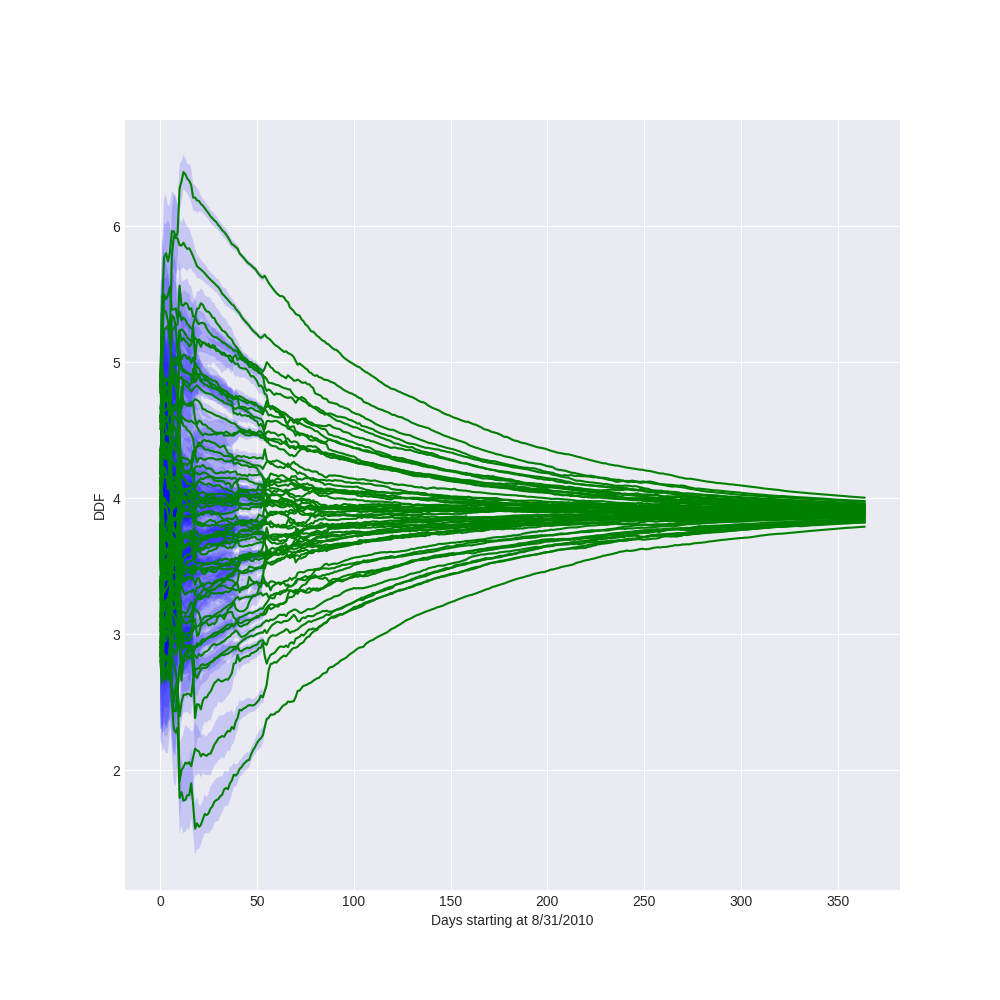
\includegraphics[width = .48\linewidth]{group17swe_ddf}} &
\subcaptionbox{Hierarchical Group 2:\texttt{pp}\label{2}}{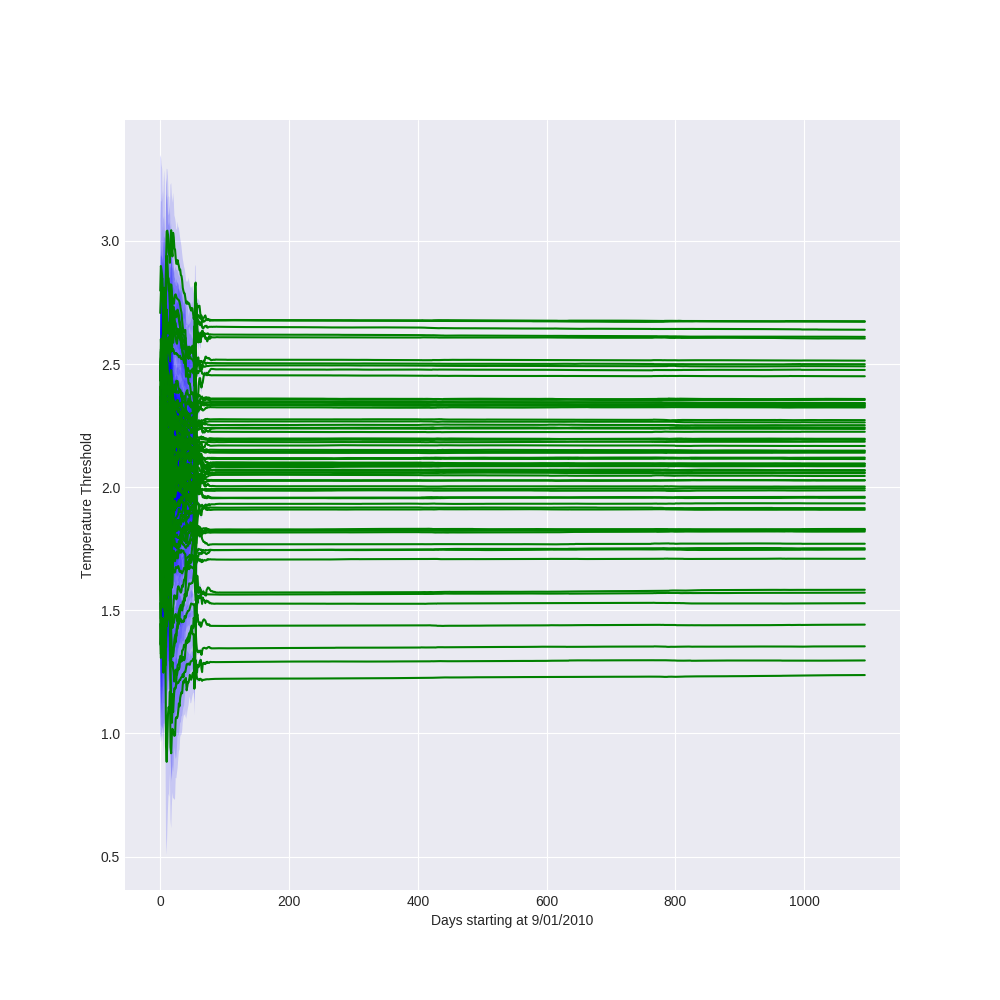
\includegraphics[width = .48\linewidth]{group17swe_pp}}

\end{tabular}
\label{fig:swe_params}
\captionof{figure}{All catchment parameters converging to a similar value. \texttt{a} blending value = .009}
\end{figure}

\begin{figure}
\centering
\begin{minipage}{.48\textwidth}
  \centering
  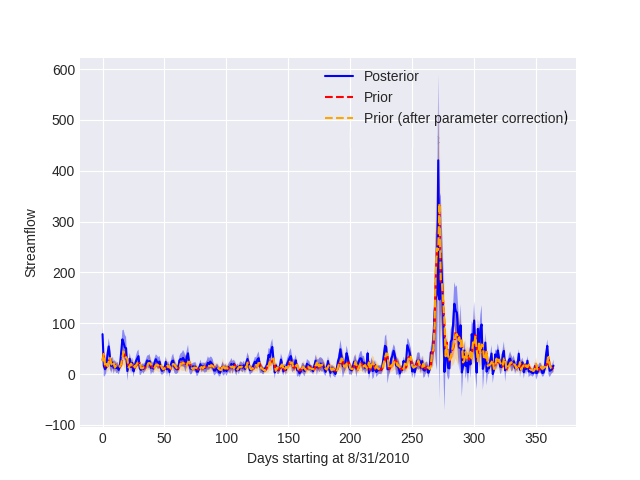
\includegraphics[width=.999\linewidth]{327str_1yr125i}
  \label{fig:327str_1yr125i}
\end{minipage}%
\begin{minipage}{.48\textwidth}
  \centering
  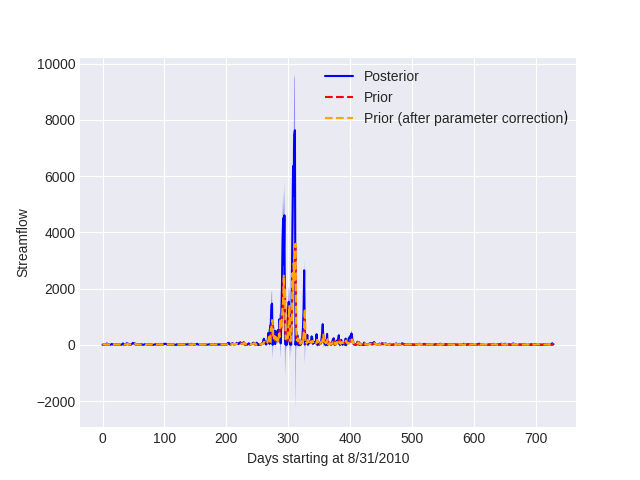
\includegraphics[width=.999\linewidth]{327str_2yr80i}
  \label{fig:327str_2yr80i}
\end{minipage}
\captionof{figure}{Ungaged catchment 327 - 125 ensemble members over 1 year (left) compared to 80 ensemble members over 2 years (right)}
\label{fig:327str_1yr2yr_compare}
\end{figure}


\section{Effects of the Hierarchical Blending Component}

To observe the effects of the hierarchical component the small dataset was used. 